% Template article for Elsevier's document class `elsarticle'
% with harvard style bibliographic references
% SP 2008/03/01

\documentclass[preprint,12pt]{elsarticle}

% Use the option review to obtain double line spacing
% \documentclass[authoryear,preprint,review,12pt]{elsarticle}

% Use the options 1p,twocolumn; 3p; 3p,twocolumn; 5p; or 5p,twocolumn
% for a journal layout:
% \documentclass[final,1p,times]{elsarticle}
% \documentclass[final,1p,times,twocolumn]{elsarticle}
% \documentclass[final,3p,times]{elsarticle}
% \documentclass[final,3p,times,twocolumn]{elsarticle}
% \documentclass[final,5p,times]{elsarticle}
% \documentclass[final,5p,times,twocolumn]{elsarticle}

% if you use PostScript figures in your article
% use the graphics package for simple commands
% \usepackage{graphics}
% or use the graphicx package for more complicated commands
% \usepackage{graphicx}
% or use the epsfig package if you prefer to use the old commands
% \usepackage{epsfig}

% The amssymb package provides various useful mathematical symbols
\usepackage{amssymb}
\usepackage{amsmath}
\usepackage{amsthm}
\usepackage{graphicx}
% The amsthm package provides extended theorem environments
% \usepackage{amsthm}
% The lineno packages adds line numbers. Start line numbering with
% \begin{linenumbers}, end it with \end{linenumbers}. Or switch it on
% for the whole article with \linenumbers.
% \usepackage{lineno}
\newcommand{\norm}[1]{\left\lVert#1\right\rVert}
\newtheorem{claim}{Claim}[section]
\newtheorem{theorem}{Theorem}[section]
\newtheorem{lemma}{Lemma}[section]
% \linenumbers

\journal{Journal of Computational Physics}

\begin{document}

\begin{frontmatter}

% Title, authors and addresses

% use the tnoteref command within \title for footnotes;
% use the tnotetext command for theassociated footnote;
% use the fnref command within \author or \address for footnotes;
% use the fntext command for theassociated footnote;
% use the corref command within \author for corresponding author footnotes;
% use the cortext command for theassociated footnote;
% use the ead command for the email address,
% and the form \ead[url] for the home page:
% \title{Title\tnoteref{label1}}
% \tnotetext[label1]{}
% \author{Name\corref{cor1}\fnref{label2}}
% \ead{email address}
% \ead[url]{home page}
% \fntext[label2]{}
% \cortext[cor1]{}
% \address{Address\fnref{label3}}
% \fntext[label3]{}

\title{Efficient solutions to robust, semi-implicit discretizations of the Immersed Boundary Method}

% use optional labels to link authors explicitly to addresses:
% \author[label1,label2]{}
% \address[label1]{}
% \address[label2]{}
\author{Hector D. Ceniceros}%\corauthref{cor}}
\address{Department of Mathematics, University of California Santa Barbara , CA 93106}
\ead{hdc@math.ucsb.edu}
\ead{www.math.ucsb.edu/\~{}hdc}
\author{Jordan E. Fisher}%\corauthref{cor}}
\address{Department of Mathematics, University of California Santa Barbara , CA 93106}
\ead{jordan@math.ucsb.edu}
\author{Alexandre M. Roma}
\address{Departamento de Matem\'atica Aplicada, Universidade de S\~ao Paulo,
Caixa Postal 66281, CEP 05311-970, S\~ao Paulo-SP, Brasil.}
\ead{roma@ime.usp.br}
\ead{www.ime.usp.br/\~{}roma}
\begin{abstract}
% Text of abstract
The Immersed Boundary Method is a versatile tool for the investigation of flow-structure interaction.
In a large number of applications, the immersed boundaries or structures are very stiff and strong tangential
forces on these interfaces induce a well-known, severe time-step restriction for explicit discretizations.  This excessive stability constraint can be removed with fully implicit or suitable semi-implicit schemes but at a seemingly prohibitive computational cost. 
While more economical alternatives have been proposed for  special cases, 
there is a practical need for a computationally efficient approach that can be applied more broadly.
% and that does not hinder the enormous structure-building capability of the Immersed Boundary methodology.  
Recently,  a robust  semi-implicit discretization introduced by Peskin in the late 70's has received renewed attention. This discretization, in which the spreading and interpolation operators are lagged,  leads to  a linear system of equations for the interface configuration at the future time when the interfacial force is linear.  However, this linear system is large and dense and thus it is challenging to streamline its solution. Moreover, while  the same linear system or one of similar structure could potentially be used in Newton-type iterations, nonlinear and highly stiff immersed structures pose additional challenges to iterative methods.
In this work,  we address these problems and propose cost-effective computational strategies  for solving Peskin's lagged-operators
type of discretization.  We do this by first constructing a sufficiently accurate approximation to the system's matrix which can
be expeditiously obtained by using a combination of pre-computed values and interpolation.  The availability  of  a matrix allows for
more efficient matrix-vector products and facilitates the design of effective iterative schemes.    
We then propose effective iterative methods to deal with both linear and nonlinear interfacial forces and simple or complex immersed structures with tethered or untethered points.  One of these iterative approaches employs a splitting in which 
we first solve a linear problem  for the interfacial force and then we use a nonlinear iteration to find the interface configuration corresponding to this force.  We demonstrate that our approach is several orders of magnitude more efficient than the standard explicit method. In addition to considering the standard elliptical drop test case, we show both the robustness and efficacy of our proposed methodology with a challenging application of a 2D model of a heart valve.
adfzzzz zxc  
\end{abstract}

\begin{keyword}
% keywords here, in the form: keyword \sep keyword
semi-implicit method \sep Stokes flow \sep Navier-Stokes equations \sep heart valve \sep multigrid
% PACS codes here, in the form: \PACS code \sep code

% MSC codes here, in the form: \MSC code \sep code
% or \MSC[2008] code \sep code (2000 is the default)

\end{keyword}

\end{frontmatter}

% main text
\section{Introduction}
The Immersed Boundary (IB) Method introduced by Peskin~\cite{Peskin77} is a versatile tool for simulating flow-structure interaction for a wide range of applications.  The IB Method employs a Lagrangian representation of 
the immersed structures and their interfacial forces and an Eulerian description of the 
flow variables (velocity and pressure).  The Lagrangian description of the immersed boundaries provides a vast structure-building capability while the Eulerian flow description permits the use of efficient flow solvers.
The power of the IB method lies in a seamless connection of the two descriptions by the use of two operations: 
{\em spreading} (of interfacial forces) and {\em interpolation} (of velocity at the immersed boundary), both achieved via mollified delta functions. 
  
In a large number of applications, the immersed boundaries or structures are very stiff and strong tangential
forces on these interfaces induce severe time-step restrictions for explicit discretization~\cite{SW95,SW99}. Fully implicit discretizations and some suitable semi-implicit schemes remove this hindering constraint but seemingly at a cost that makes these options impractical~\cite{TP92, MP93}.  A very economical semi-implicit method has been proposed recently by Hou and Shi~\cite{HS2008a,HS2008b}. This novel approach relies on an ingenious  small scale decomposition and becomes explicit in Fourier space. While nearly computationally optimal, the method of Hou and Shi is applicable only to a simple interface, given as a closed curve. Thus, there is still a practical need for a robust, cost-effective approach that can be applied more broadly; one that can be used
for immersed structures of complex geometry, composed of mix tethered and untethered links,  which are required in many of the applications of the IB Method.  The advancement of such an approach is the main focus of this work.

Our starting point is a semi-implicit scheme introduced Peskin~\cite{Peskin77} in the late 70's, in which
the spreading and interpolation operators are lagged, i.e. evaluated at the current interfacial configuration rather than at the future one.  Variations of this scheme were also considered by Tu and Peskin~\cite{TP92} and by Mayo and Peskin~\cite{MP93}. This lagged-operators discretization has recently received renewed attention.  In particular, Newren, Fogelson, Guy, and Kirby
proved that this scheme, in its first order or second order Crank-Nicolson form, is unconditionally stable when inertia is neglected and the interfacial  force is linear and self-adjoint~\cite{NFGK2007}. Numerical experiments in ~\cite{NFGK2007}, as well as our own experiments, suggest this stability extends to the inertial case with nonlinear interfacial force. Thus, it is now established that 
Peskin's original semi-implicit discretization enjoys great stability properties and robustness, 
hence the relevant question is whether its solution  can be computed at a reasonable cost. Recently, Mori and Peskin~\cite{MP2008}  took an important step to answer this question. 
They considered a variation of this scheme, with a linearized tension force discretization which leads to a linear system of equations for the interface configuration at the future time step. They also considered a fully implicit method solved iteratively where each of the iterates has the same structure as the linearized semi-implicit discretization.  Mori and Peskin opted for Krylov subspace methods to solve the linear system to take advantage of the  fact that matrix-vector products can be obtained via standard operations in the IB method and to avoid the construction of the system's dense matrix. 

In this work  we demonstrate that the solution to Peskin's operator-lagged discretization
can be obtained much more efficiently by working directly with the matrix, and by using suitable linear and nonlinear iterative methods. More precisely, we construct a sufficiently accurate approximation to the matrix which can
be expeditiously obtained by using a combination of pre-computed values and interpolation.   The availability  of a matrix allows 
for streamlined matrix-vector products and facilitates the design of effective iterative schemes.   Most of the work to date on the investigation and removal of the numerical stiffness of the IB Method has focused on a simple test problem: a relaxing elliptical drop.
While this test model contains the characteristic high stiffness of the IB approach in a simple interfacial geometry it does not showcase the additional complications that might arise when the immersed structure is composed of crossed links with both tethered and untethered points. Such complex structures are common in applications, starting with the origins of the method to investigate blood
flow in the heart~\cite{Peskin77}.  In this work, in addition to obtaining efficient methods for 
the standard elliptical drop test case, we also propose cost-effective iterative methods to deal with cases of complex immersed structures with tethered and untethered points. In our proposed approach
we employ  a splitting in which we first solve efficiently a linear problem for the interfacial force and then we use a fast-converging nonlinear iteration to find the interface configuration corresponding to this force.  We develop this method in the context of a 2D
model of a heart valve and demonstrate that our approach is several orders of magnitude more efficient than the standard explicit method. 
 
 The rest of the paper is organized as follows. In Section~\ref{Sec:IB}, we review the formulation of the IB method. Section~\ref{Sec:discretization} deals with the discretization with the focus on  Peskin's semi-implicit scheme with lagged-operators. We devote Section~\ref{Sec:matrix} to the construction of the approximation to the matrix and we obtain an estimate for that approximation.
 In Section~\ref{Sec:drop}, we consider the case of the relaxing elliptical drop with both linear and nonlinear forces.  Section~\ref{Sec:valve} is devoted to the heart valve problem and the splitting scheme.


 \section{The Immersed Boundary Method}
 \label{Sec:IB}
To describe the method,  in its simplest form, we 
consider a two-dimensional, incompressible, Newtonian fluid occupying a domain $\Omega \subset \mathbb{R}^2$. Inside this domain
we assume that there is an immersed, neutrally buoyant, elastic structure (also referred to as boundary or interface). This fluid-immersed interface is composed of a system  $\Gamma$ of elastic fibers whose position at any time $t$ is represented in Lagrangian form by $\mathbf{X}(s,t)$, where $s \in B$ is a Lagrangian parameter. The interface $\Gamma$
need not be closed or even continuous. The governing equations are:
\begin{align}
\rho \left(\frac{\partial \mathbf{u}}{\partial t} + \mathbf{u}\cdot\nabla\mathbf{u} \right) &= -\nabla p + \mu\nabla^2 \mathbf{u} + \mathbf{f}, \label{eq:momentum}\\ 
\nabla \cdot \mathbf{u} &= 0, \label{eq:incompressibility}\\
\frac{\partial \mathbf{X}}{\partial t}  &= \mathbf{u}(\mathbf{X},t), \label{eq:noslip}
\end{align}
where $\rho$ and $\mu$ are the density and viscosity, respectively (both assumed to be constant). Here $\mathbf{u}(\mathbf{x},t)$ and $p(\mathbf{x},t)$ are the velocity field and the pressure, respectively, described in terms of the Eulerian, Cartesian coordinate $\mathbf{x}$. The term $\mathbf{f}$ represents the singularly supported interfacial (tension) force of the immersed structure acting onto the fluid. The system (\ref{eq:momentum})-(\ref{eq:noslip}) is supplemented with initial and boundary conditions. Throughout this work, we consider only periodic boundary conditions and $\Omega$ is a rectangular domain.

The crux of the IB method and much of its versatility is the seamless connection of the Lagrangian representation of the immersed structure with the Eulerian representation of the flow. This is achieved via the identities:
\begin{align}
\frac{\partial \mathbf{X}}{\partial t}  &= \int_{\Omega} \mathbf{u}(\mathbf{x},t)\delta(\mathbf{x}-\mathbf{X}(s,t)) d \mathbf{x}, \label{eq:cont_interp} \\
\mathbf{f}(\mathbf{x},t) &= \int_{B} \mathbf{F}(\mathbf{X}(\cdot,\cdot)s,t)\delta(\mathbf{x}-\mathbf{X}(s,t)) ds
\label{eq:cont_spread},
\end{align}
where $\delta$ denotes the (two-dimensional) Dirac delta distribution. In (\ref{eq:cont_spread}), $\mathbf{F}$
represents the elastic force density of $\Gamma$ and is described in Lagrangian coordinates.  For example, 
if the tangent direction $\mathbf{t}$ along the fibers varies smoothly and if the local elastic energy density is assumed to depend only on the tangential strain $|\frac{\partial\mathbf{X}}{\partial s}|$ then
\begin{equation}
\mathbf{F}(\mathbf{X},s,t) = \frac{ \partial }{\partial s} \left(T\left(\left|\frac{\partial\mathbf{X}}{\partial s}\right|\right) \mathbf{t}\right).
\end{equation}
Here $T(|\frac{\partial\mathbf{X}}{\partial s}|)$ is the fiber (interfacial) tension and $\mathbf{t}$ is the unit tangent,
\begin{equation}
\mathbf{t} =\frac{\frac{\partial\mathbf{X}}{\partial s}}{|\frac{\partial\mathbf{X}}{\partial s}|}.
\end{equation}
Thus $\mathbf{F}$ is in general a nonlinear function of the interfacial configuration. We denote this relation by
\begin{equation}
\mathbf{F} = \mathcal{A}(\mathbf{X}).
\end{equation}





\section{Discretization}
\label{Sec:discretization}
We consider uniform Cartesian grids $\mathcal{G}_\Omega$  and $\mathcal{G}_B$ with grid size $h$ and $h_B$
to discretize $\Omega$ and $B$ respectively and employ standard second order finite differences for the spatial derivatives.  We write Peskin's original semi-implicit discretization in the form
\begin{align}
\rho\left(\frac{\mathbf{u}^{n+1}-\mathbf{u}^n}{\Delta t} + \mathbf{u}^n\cdot\mathbf{D}_h\mathbf{u}^n\right) &= -\mathbf{D}_h p^{n+1}+ \mu L_h \mathbf{u}^{n+1} + \mathcal{S}_n\mathcal{A}_{h_B}(\mathbf{X}^{n+1}), \label{eq:dmoment} \\
\mathbf{D}_h \cdot \mathbf{u}^{n+1} &= 0, \label{eq:ddivergence} \\
\frac{\mathbf{X}^{n+1}-\mathbf{X}^n}{\Delta t} &= \mathcal{S}^*_n\mathbf{u}^{n+1}, \label{eq:Xt}
\end{align}
where a superscript  $m$ denotes a numerical approximation taken at the time $m \Delta t$ and $\Delta t$ is the time step. The spatial operators $\mathbf{D}_h$ and $L_h$ are the standard second order approximations to the gradient and the laplacian, respectively,  and $\mathcal{A}_{h_B}$ is a suitable discrete version of $\mathcal{A}$. 

  $ \mathcal{S}_n$ and $ \mathcal{S}^*_n$ are the  {\em lagged} spreading and interpolation operators, respectively,  given by
\begin{align}
(\mathcal{S}_n G) (\mathbf{x})&= \sum_{s \in \mathcal{G}_B }G(s) \delta_h(\mathbf{x}-\mathbf{X}^n(s))h_B,
\label{eq:S} \\
(\mathcal{S}^*_n w)(s) &= \sum_{ \mathbf{x} \in \mathcal{G}_\Omega} w(\mathbf{x})\delta_h(\mathbf{x}-\mathbf{X}^n(s))h^2,
\label{eq:S*}
\end{align}
where $\delta_h(\mathbf{x}) = d_h(x)d_h(y)$ and $d_h$ is an approximation of the one-dimensional delta. 
These operators are called lagged because the interface configuration $\mathbf{X}^n$ is used 
instead of the future configuration $\mathbf{X}^{n+1}$.

There is flexibility in the choice of $d_h$ but for concreteness in the presentation we choose Peskin's 
delta~\cite{Peskin77}:
\begin{equation}
\delta_h(r) = \begin{cases}
\frac{1}{4h}\left( 1+\cos(\frac{\pi r}{2h})\right)& \textrm{if } |r|\leq 2h \\
0& \textrm{otherwise}.
\end{cases}
\end{equation}

Let us rewrite (\ref{eq:dmoment}) as
\begin{equation}
\mathbf{u}^{n+1}=-\frac{\Delta t}{\rho} \mathbf{D}_h p^{n+1} + \nu\Delta t L_h \mathbf{u}^{n+1} + \mathbf{a}^{n+1},
\label{eq:upa}
\end{equation}
where $\nu=\mu/\rho$ and
\begin{equation}
\mathbf{a}^{n+1}= \frac{\Delta t}{\rho}\, \mathcal{S}_n\mathcal{A}_{h_B}(\mathbf{X}^{n+1})+\mathbf{u}^n-\Delta t \, \, \mathbf{u}^n \cdot \nabla_h \mathbf{u}^n. \label{eq:a}
\end{equation}
We can eliminate the pressure term in (\ref{eq:upa}) using (\ref{eq:ddivergence}) by introducing a discrete projection
$P_h$ defined as 
\begin{equation}
\mathbf{v} = P_h \mathbf{v} + \mathbf{D}_h \phi_v, \qquad \mathbf{D}_h \cdot P_h \mathbf{v} =0, \qquad P_h \mathbf{D}_h \phi_v=0.
\end{equation}
for any smooth vector field $\mathbf{v}$ defined on the grid $\mathcal{G}_{\Omega}$. Applying $P_h$ to (\ref{eq:upa}), using  (\ref{eq:ddivergence}) and that for periodic boundary conditions $L_h$ and $P_h$ commute we get
\begin{equation}
\mathbf{u}^{n+1}= \nu\Delta t L_h \mathbf{u}^{n+1} + P_h \mathbf{a}^{n+1},
\end{equation}
that is
\begin{equation}
\mathbf{u}^{n+1} = (I -\nu\Delta t L_h)^{-1}  P_h \mathbf{a}^{n+1}.
\end{equation}
Let us denote
\begin{equation}
\mathcal{L}_h = (I -\nu\Delta t L_h)^{-1}  P_h. \label{eq:L_h}
\end{equation}
$\mathcal{L}_h$ is a linear operator which henceforth we will refer to as the fluid solver. Note that with periodic boundary conditions and a standard second order finite difference approximation for the spatial derivatives,
  $I -\nu\Delta t L_h$ is symmetric and positive definite and as a result so is its inverse. 
  On the other hand, $P_h$ is also symmetric and, being 
  a projection, it is positive semi-definite. Moreover, $P_h$ and $(I -\nu\Delta t L_h)^{-1}$ commute 
  as can be shown using the discrete Fourier transform. Consequently, these two symmetric operators can be diagonalized by the same orthogonal matrix and thus the product, $\mathcal{L}_h $, is positive semi-definite. 





Using this notation Peskin's semi-implicit method  can be encoded as
\begin{align}
\mathbf{u}^{n+1} &= \mathcal{L}_h \mathbf{a}^{n+1}, \label{eq:uL} \\
\mathbf{X}^{n+1}&=\mathbf{X}^n +\Delta t\mathcal{S}^*_n\mathbf{u}^{n+1}, \label{eq:Xu}
\end{align}
where $ \mathbf{a}^{n+1}$ is given by (\ref{eq:a}). Eliminating $\mathbf{u}^{n+1}$ in (\ref{eq:Xu}) we obtain  a system of equations for the immersed boundary configuration $\mathbf{X}^{n+1}$:
\begin{equation}
\mathbf{X}^{n+1} = \mathcal{M}_n\mathcal{A}_{h_B} (\mathbf{X}^{n+1}) + \mathbf{b}^n, \label{eq:Xnl}
\end{equation}
where 
\begin{equation}
 \mathcal{M}_n =  \alpha \,  \mathcal{S}^*_n \mathcal{L}_h \mathcal{S}_n,
\end{equation}
with
\begin{equation}
\alpha = \frac{(\Delta t)^2}{\rho}
\end{equation}
and 
\begin{equation}
 \mathbf{b}^n = \mathbf{X}^n + \Delta t \mathcal{S}^*_n \mathcal{L}_h [\mathbf{u}^n-\Delta t \mathbf{u}^n \cdot
 \nabla_h \mathbf{u}^n]. \label{eq:bn}
\end{equation}
We have thus reduced (\ref{eq:dmoment})-(\ref{eq:Xt}) to a single system of  equations involving only the unknown $\mathbf{X}^{n+1}$. If the number of Lagrangian nodes is $N_B$ then (\ref{eq:Xnl}) represents a system of $2N_B$ equations for the 
$2N_B$ values $\mathbf{X}^{n+1}=(X^{n+1},Y^{n+1})$. If we can solve this system then we can obtain $\mathbf{u}^{n+1}$ via (\ref{eq:uL}). 


Note that  the positive semi-definiteness of $\mathcal{L}_h$ extends to $\mathcal{M}_n$. Indeed, if we define the inner product on $\Omega$ as
\begin{align}
(u,v)_{\Omega} &= \sum_{\mathbf{x} \in \mathcal{G}_\Omega} u(\mathbf{x})v(\mathbf{x})h^2,\label{eq:innero} \\
(\mathbf{u},\mathbf{v})_{\Omega} &=  (u_1,v_1)_{\Omega} + (u_2,v_2)_{\Omega},
\end{align}
and on $B$ as
\begin{align}
(F,G)_{B} &= \sum_{\mathbf{x} \in \mathcal{G}_B} F(\mathbf{x})G(\mathbf{x})h_B,\label{eq:innerb} \\
(\mathbf{F},\mathbf{G})_{B} &= (F_1,G_1)_{B} + (F_2,G_2)_{B},
\end{align}
then  $\mathcal{S}_n$ and $\mathcal{S}_n^*$ as given in (\ref{eq:S})-(\ref{eq:S*}) are adjoints to each other 
and
\begin{align}
( \mathbf{F}, \mathcal{M}_n\mathbf{F} )_{B} &= \alpha ( \mathbf{F},\mathcal{S}^*_n\mathcal{L}_h\mathcal{S}_n \mathbf{F})_{B} =\alpha ( \mathcal{S}_n\mathbf{F}, \mathcal{L}_h\mathcal{S}_n\mathbf{F})_{B}\geq 0.
\end{align}
In fact, $( \mathbf{F}, \mathcal{M}_n\mathbf{F} )_{B}>0$ for $\mathbf{F} \neq 0$ unless the Eulerian force $\mathcal{S}_n \mathbf{F}$ is in the kernel of the projection, i.e. if it is a gradient field,  or if there are too many Lagrangian points per Eulerian cell and injectivity of $\mathcal{S}_n$ is lost. There are physical situations, such as for example a circular drop under uniform surface tension at equilibrium, where the Eulerian force is a gradient field at the continuous level (to balance the gradient of the pressure). However, as it is well 
known, the IB method spreading of the force fails in general to produce a discrete gradient which results in the generation of non-zero velocities referred to as spurious currents~\cite{Tryg01}.  Ironically, this defect of the IB approach has the benefit of rendering  $ \mathcal{M}_n$ positive definite provided $\mathcal{S}_n$ remains injective. This is something that we will exploit via {\em multigrid}.


The focus of this paper is to propose efficient methods for solving (\ref{eq:Xnl}) to be able to remove the severe numerical stiffness of the IB method in an economical and robust fashion for a wide range of practical flow-structure situations.  Of course, to be efficient the specific computational approach  has to be dependent on the geometry of the immersed structure and the force operator $\mathcal{A}_{h_B}$.  This is something that has been largely 
overlooked in the literature as the research has concentrated mostly on understanding  and removing the stiffness 
on the simplest setting: a simple closed (elliptical) interface with a linear density force $\mathcal{A}_{h_B}$.
Here, we consider both linear and nonlinear $\mathcal{A}_{h_B}$ with simple and complex immersed structure geometries to highlight the challenges in producing efficient solvers and to illustrate our proposed approaches.


\section{Some comments on computational costs and efficiency} 
\label{Sec:Costs}
One of the most commonly used schemes with an explicit treatment of the immersed boundary is the 
so-called Forward Euler/Backward Euler (FE/BE)~\cite{SW99} in which the tension force is explicit (Forward Euler) and the 
viscous term is implicit (Backward Euler). That is,
\begin{align}
\mathbf{u}^{n+1} &= \mathcal{L}_h \left[\frac{\Delta t}{\rho}\, \mathcal{S}_n\mathcal{A}_{h_B}(\mathbf{X}^{n})+\mathbf{u}^n-\Delta t \, \, \mathbf{u}^n \cdot \nabla_h \mathbf{u}^n\right], \label{eq:FE} \\
\mathbf{X}^{n+1}&=\mathbf{X}^n +\Delta t\mathcal{S}^*_n\mathbf{u}^{n+1}. \label{eq:BE}
\end{align}
The main cost of this scheme per time step is the fluid solver, i.e the operation involving $\mathcal{L}_h$.  On the other hand
any solution method for (\ref{eq:Xnl}) requires the evaluation of $\mathbf{b}^n$, given by (\ref{eq:bn}), and thus  at
least one fluid solver operation. Hence, it seems appropriate to measure the cost of iterative methods for (\ref{eq:Xnl}) relative to that 
of one FE/BE time-step and we will refer to this unit as one FE/BE. 
Our goal is to present robust solution methods to (\ref{eq:Xnl}) that have cost of just a few FE/BE's. Naturally, 
because the semi-implicit scheme allows for time steps several orders of magnitude larger than those permitted by FE/BE in a stiff problem,  the extra computational work per time step will be more than compensated and a speed-up of several magnitudes could be achieved. 

In the design of efficient iterative methods for (\ref{eq:Xnl}) it is crucial to streamline the calculation of quantities of the form
$\mathcal{M}_n\mathbf{F}$. These quantities can be computed in two ways.  Given an interface-defined vector $\mathbf{F}$
we can apply in sequence the operations of spreading, fluid solver, and interpolation. Alternatively,  we can construct a matrix representation of $\mathcal{M}_n$ and use matrix-vector multiplication.  Given that a direct computation of the matrix
is prohibitively expensive, $Nb \times FE/BE$, all related work to date has avoided the latter approach.  However, 
there are some advantages of having a matrix representation of $\mathcal{M}_n$ and, as we show in the next section,  it is possible to
construct a sufficiently accurate approximation to the matrix in only $O(FE/BE)$ operations.

One of the advantages of having a matrix representation of the operator $\mathcal{M}_n$ is that we can gain access to  a wider range of iterative methods.  Multigrid smoothers like Gauss-Seidel or S.O.R., which are inaccessible with the spreading-fluid solver-interpolation approach, could be easily implemented if the matrix  is available.
Also, multigrid-based methods are greatly simplified when we have a matrix representation of $\mathcal{M}_n$, which allows us to employ a straightforward algebraic multigrid as opposed to a geometric one. One of the more subtle issues with using a geometric multigrid is how to coarsen the Eulerian grid. Uniform coarsening would be ineffective for example in the case of our heart valve model 
 because as we coarsen the valve geometry there remain points close together which would require a fine Eulerian mesh to resolve, see Fig.~\ref{fig:Valve1}. If a geometric multigrid were to be employed we would need to implement adaptive coarsening.
 
 A second advantage of having a matrix representation of $\mathcal{M}_n$ is that we can obtain direct solutions of {\em coarse} (small) linear systems of the form $\mathcal{M}_n\mathbf{F}=\mathbf{Z}$ which could be useful in a number of situations; an instance of this will be discussed later in the context of the heart valve problem. But perhaps the main advantage is that of cost when 
 computing quantities of the form  $\mathcal{M}_n\mathbf{F}$.  If this matrix-vector product is computed via the operator sequence  spreading-fluid solver-interpolation the cost is about one FE/BE or $O(N^2\log N) + O(N_B)$, when $N^2$ is the number of Eulerian nodes and the fluid solver is based on the Fast Fourier Transform (FFT).  
 On the other hand, a matrix-vector multiplication involving $\mathcal{M}_n$ requires $O(N_B^2)$ operations.  If  $N_B \sim N$ as it is typical in 2D applications, then the second approach has lower computational complexity. While
 the elimination of the factor $\log N$ might seem like a modest gain, we find that in practice (for $N_B=2N$) using the 
 matrix representation to compute matrix-vector products is significantly faster  than the spreading-fluid solver-interpolation approach, even at modest resolutions.  Table~\ref{Table:MV} gives the CPU time in units of FE/BE (average CPU time of one FE/BE time-step for a given $N\times N$ Eulerian grid and $N_B=2N$) for matrix-vector multiplications computed using a matrix representation of  $\mathcal{M}_n$.  For example, at $N_B=1024$,  the computation of a matrix-vector product with this approach is $1/71$ FE/BE, i.e.
  71 times faster than it would be using the spreading-fluid solver-interpolation option.
  If in addition,  we take into the account that many matrix-vector products are needed in the course of an iterative method then the computational savings are significant. We note however that as the ratio $N_B/N$ increases the savings get reduced and the computational advantage of using the matrix to obtain the product could be lost eventually. For example, in our application of the heart valve model where $N_B  \sim 4N$, the speedup in using the matrix form drops to roughly $10$ at moderate to fine resolutions. While not as dramatic as that in the $N_B=2N$ case, it still leads to substantial savings in the overall algorithm.  However, 
  in a fully 3D application with a 2D immersed membrane we would have $N_B \sim N^2$ leading to a cost of  $O(N^4)$ for 
   a matrix-vector multiplication using the matrix  while obtaining the same product via spreading-fluid solver-interpolation would be $O(N^3\log N)$. 
  
% \begin{table}
%\caption{Average CPU time in seconds for a FE/BE timestep with given $N$ on a square $N\times N$ Eulerian grid}
%\label{table:FEBEcost}
%\begin{center}
%\begin{tabular}{|c|c c c c c|}
%\hline
%$N$ & 128 & 256 & 384 & 512 & 640\\
%\hline
%\textrm{FE/BE} & .0201 & .134 & .365 & .725 & 1.04\\
%\hline
%\end{tabular}
%\end{center}
%\label{table:MatrixCost}
\begin{table}
\begin{center}
\begin{tabular}{|c|c c c|}
\hline
%$N_B$ & 128 & 256 & 384 & 512 & 640 & 768 & 896 & 1024\\
$N_B=2N$ &  256  & 512 & 1024\\
\hline
\textrm{Matrix-Vector product} 
& 1/26.8  & 1/58 &  1/71\\
%\hline
%\textrm{Matrix construction} &
%.00631 & .02030 & .03582 & .07347 & .10686 & .15433 & .20915 & .29323\\
\hline
\end{tabular}
\end{center}
\caption{Average CPU time in FE/BE units for a matrix-vector multiplication involving $\mathcal{M}_n$ for given $N_B=2N$}
\label{Table:MV}
\end{table}


\section{An expedited computation of a matrix representation of $\mathcal{M}_n$}
\label{Sec:matrix}
\subsection{An approximation from translation invariance}
Let us consider again the linear fluid solver operator (\ref{eq:L_h}) with periodic boundary conditions. Utilizing the Fourier transform we obtain a representation formula of the form
\begin{equation}
 \mathcal{L}_h \mathbf{f}(\mathbf{x}) = \sum_{\mathbf{y} \in \mathcal{G}_\Omega} G_h (\mathbf{x}-\mathbf{y})\mathbf{f}(\mathbf{y})h^2, \qquad \text{for $\mathbf{x} \in \mathcal{G}_\Omega$},
\label{eq:G_h}
\end{equation}
where the Green function $ G_h (\mathbf{x}-\mathbf{y})$ is a $2 \times 2$ matrix with vanishing zero Fourier mode. 

Recall that $\mathcal{M}_n =  \alpha \,  \mathcal{S}^*_n \mathcal{L}_h \mathcal{S}_n$, thus its entries  $(\mathcal{M}_n)_{ij}$ 
correspond to $\alpha$ times  the velocity that is obtained by {\em interpolating}  
the values produced at a given interfacial node $\mathbf{X}_i$ by  {\em spread} unit horizontal and vertical forces located at another immersed boundary node  $\mathbf{X}_j$. For the continuum  problem this velocity depends only on the difference 
$\mathbf{X}_j - \mathbf{X}_i$ but due to the spreading and interpolation operators this translation invariance is not exact at the discrete level. However, as we prove later, we can still obtain sufficiently accurate approximations to  $(\mathcal{M}_n)_{ij}$  by assuming translation invariance with the added benefit of a dramatic cost reduction.
Specifically, we propose to approximate $(\mathcal{M}_n)_{ij}$  with values obtained  by shifting both $\mathbf{X}_i$ and $\mathbf{X}_j$ an equal amount such that $\mathbf{X}_j$ lies exactly on an Eulerian node, which we may take as the origin. That is, we can fix the point (the origin) at which unit horizontal and vertical forces are applied (and spread) and then evaluate the effects everywhere else on the Eulerian grid by  applying just {\em two} fluid solves: one each for a horizontal and vertical force at the origin. These Eulerian grid values can be pre-computed at the
beginning of the simulation and then be used as a look-up table to obtain the corresponding values at 
any interfacial point $\mathbf{X}_i$  via standard interpolation. The generation of the one-time lookup table is only two $FE/BE$ and
the interpolation to generate the approximation of  $\mathcal{M}_n$ is only $O(N_B^2)$.

We proceed now to detail the computation of $\mathcal{M}_n$.  
%%%%%%%%%%%%%%%%%%%%%%%%%%%%%%%%%%%
Define for each interfacial node $j$, $1 \leq j \leq N_B$, the unit forces
\begin{align}
\mathbf{f}^j_k = 
\begin{cases}
(0,0)
 & \text{If $k \neq j$}, \\
\mathbf{e}_1 & \text{If $k=j$}
\end{cases} \qquad 1 \leq k \leq N_B \label{eq:f}
\end{align}
and
\begin{align}
\mathbf{g}^j_k =
\begin{cases}
(0,0)
 & \text{If $k \neq j$}, \\
\mathbf{e}_2 & \text{If $k=j$}
\end{cases} \qquad 1 \leq k \leq N_B, \label{eq:g}
\end{align}
where $\mathbf{e}_1=(1,0)$ and $\mathbf{e}_2=(0,1)$.
Then
\begin{align}
(\mathcal{M}_n \mathbf{f}^j)_i &=
\left( \alpha \,  \mathcal{S}^*_n \mathcal{L}_h 
\sum_{\mathbf{X}_k \in \mathcal{G}_B}  \mathbf{f}^j_k \delta_h (\mathbf{x}-\mathbf{X}_k) h_B \right)_i  \\
&= \alpha  h_B \left(  \mathcal{S}^*_n \mathcal{L}_h   \mathbf{e}_1 \delta_h (\mathbf{x}-\mathbf{X}_j)  \right)_i \\
&=\alpha h_B  \, \sum_{\mathbf{z} \in \mathcal{G}_\Omega} \left(\mathcal{L}_h   \mathbf{e}_1 \delta_h (\mathbf{x}-\mathbf{X}_j) \right)
(\mathbf{z}) \delta_h(\mathbf{z}-\mathbf{X}_i)h^2 \\
& \approx  \alpha h_B  \, \sum_{\mathbf{z} \in \mathcal{G}_\Omega} \left( \mathcal{L}_h   \mathbf{e}_1 \delta_h (\mathbf{x}) \right) (\mathbf{z})
\delta_h\left(\mathbf{z}-(\mathbf{X}_i-\mathbf{X}_j)\right)h^2,
\end{align}
and similarly
\begin{align}
(\mathcal{M}_n \mathbf{g}^j)_i  & \approx  \alpha h_B  \, \sum_{\mathbf{z} \in \mathcal{G}_\Omega} \left( \mathcal{L}_h   \mathbf{e}_2 \delta_h (\mathbf{x}) \right) (\mathbf{z})
\delta_h\left(\mathbf{z}-(\mathbf{X}_i-\mathbf{X}_j)\right)h^2.
\end{align}
With these two approximations we define the vector-valued functions
\begin{align}
\mathbf{T}(\mathbf{y}) &=  \alpha h_B \, \sum_{\mathbf{z} \in \mathcal{G}_\Omega} \left(  \mathcal{L}_h \mathbf{e}_1 \delta_h (\mathbf{x}) \right) (\mathbf{z}) \delta_h\left(\mathbf{z}-\mathbf{y}\right)h^2, \\
\mathbf{U}(\mathbf{y}) &=  \alpha h_B \, \sum_{\mathbf{z} \in \mathcal{G}_\Omega}  \left( \mathcal{L}_h \mathbf{e}_2 \delta_h (\mathbf{x}) \right) (\mathbf{z}) \delta_h\left(\mathbf{z}-\mathbf{y}\right)h^2,
 \end{align}
 and note that
 \begin{align}
(\mathcal{M}_n \mathbf{f}^j)_i & \approx \mathbf{T}(\mathbf{X}_i -\mathbf{X}_j), \label{eq:Mf}\\
(\mathcal{M}_n \mathbf{g}^j)_i & \approx \mathbf{U}(\mathbf{X}_i -\mathbf{X}_j). \label{eq:Mg}
\end{align}
We can now compute the entries of a matrix representation of the linear operator $\mathcal{M}_n$ from $\mathbf{T}$ and 
$\mathbf{U}$. To this end, we write the configuration $\mathbf{X}$ of the discretized immersed structure as the $2N_B$-array 
\begin{equation}
\mathbf{X}=\begin{bmatrix} X \\ Y \end{bmatrix} =
 \begin{bmatrix} X_1 \\ \vdots \\ X_{N_B} \\Y_1 \\ \vdots \\Y_{N_B}
\end{bmatrix} ,
\end{equation}
and similarly we write  $\mathbf{F}=\mathcal{A}_{h_B}(\mathbf{X})=(F,G)^T$. We seek then four $N_B\times N_B$ matrices $A$, $B$, $C$, and $D$ such that
\begin{equation}
\mathcal{M}_n\mathbf{F} =
\begin{bmatrix}
A & B \\
C & D \end{bmatrix}
\begin{bmatrix}
F  \\
G \end{bmatrix} . \label{eq:ABCD}
\end{equation}
Then from (\ref{eq:Mf})-(\ref{eq:Mg}) and the definition of the interfacial point forces (\ref{eq:f})-(\ref{eq:g}), it follows that
\begin{align}
\begin{bmatrix} A_{ij} \\ C_{ij} \end{bmatrix}
&\approx \mathbf{T}(\mathbf{X}_i-\mathbf{X}_j),
\end{align}
and
\begin{align}
\begin{bmatrix} B_{ij} \\ D_{ij} \end{bmatrix}
&\approx \mathbf{U}(\mathbf{X}_i-\mathbf{X}_j).
\end{align}
The domain of both $\mathbf{T}$ and $\mathbf{U}$ is $\Omega$. To expedite the calculation we precompute both functions on the Eulerian grid $\mathcal{G}_\Omega$. The value of $\mathbf{T}$ or $\mathbf{U}$ at any other point is obtained via simple linear
interpolation from the corresponding grid values. Thus, each evaluation of $\mathbf{T}$ or $\mathbf{U}$  costs only $\mathcal{O}(1)$  and consequently, we construct in 
this manner  the entire matrix representation of $\mathcal{M}_n$ with an optimal $\mathcal{O}(N_B^2)$ cost.
Table~\ref{Table:MConstruct} gives the CPU time to obtain the matrix in units of FE/BE, when $N_B=2N$. 
\begin{table}
\begin{center}
\begin{tabular}{|c|c c c|}
\hline
%$N_B$ & 128 & 256 & 384 & 512 & 640 & 768 & 896 & 1024\\
$N_B=2N$ &  256  & 512 & 1024 \\
\hline
\textrm{Matrix construction} 
& 1/3.3  & 1/1.8 &  1/2.5 \\
\hline
\end{tabular}
\end{center}
\caption{Average CPU time in FE/BE units to construct the matrix approximation to $\mathcal{M}_n$ for given $N_B=2N$}
\label{Table:MConstruct}
\end{table}

\subsection{Error estimate for approximation of the matrix representation of $\mathcal{M}_n$}
We proceed to prove the error introduced via approximation in the above construction of $\mathcal{M}_n$ is negligible. In what follows we assume our domain $\Omega = [0,1]\times[0,1]$ and define $\mathcal{G}_F$ to be a uniform Cartesian grid with grid size $2\pi h$ to discretize $[0,2\pi)\times[0,2\pi)$. $\mathcal{G}_F$ is the discrete Fourier space associated with $\mathcal{G}_h$.
We first require a bound on $G_h$, the Green's function used in (\ref{eq:G_h}). Given the vector fields
\begin{equation}
\mathbf{g}_1(\mathbf{x}) = \begin{cases}
(1/h^2,0)& \textrm{if } \mathbf{x} = \mathbf{0} \\
(0,0)& \textrm{otherwise}
\end{cases}
\end{equation}
and
\begin{equation}
\mathbf{g}_2(\mathbf{x}) = \begin{cases}
(0,1/h^2)& \textrm{if } \mathbf{x} = \mathbf{0} \\
(0,0)& \textrm{otherwise}
\end{cases}
\end{equation}
defined for $\mathbf{x} \in \mathcal{G}_\Omega$, 
$G_h$ is a $2\times 2$ matrix valued function given by
\begin{equation}
G_h(\mathbf{x})=
\left( \begin{array}{cc}
u_1(\mathbf{x}) & u_2(\mathbf{x}) \\
v_1(\mathbf{x}) & v_2(\mathbf{x})
\end{array} \right),
\end{equation}
where $(u_1,v_1) = \mathcal{L}_h(\mathbf{g}_1)$ and $(u_2,v_2) = \mathcal{L}_h(\mathbf{g}_2)$.

We make the following claims about the four components of $G$.
\begin{lemma}
If $\Delta t$ is proportional to $h$ then the $\sup$ norm of each component of $G_h$ over $\mathcal{G}_\Omega$ scales asymptotically like $\mathcal{O}({\Delta t}^{-1}\log(h^{-1}))$.
\end{lemma}
\begin{proof}
By definition
\begin{equation}
(u_1,v_1) = (I -\nu\Delta t L_h)^{-1}  P_h (\mathbf{g}_1 / h^2).
\end{equation}
In Fourier space $|\widehat{P_h (\mathbf{g}_1)}(\mathbf{\xi})| = |\hat{\mathbf{g}}_1(\mathbf{\xi})-|\hat{D}_h|^{-2}\hat{D}_h\hat{D}_h\cdot\hat{\mathbf{g}}_1(\mathbf{\xi})| \leq |\hat{\mathbf{g}}_1(\mathbf{\xi})| = 1/h^2$, for $\mathbf{\xi} \in \mathcal{G}_F$. This follows easily from a direct calculation or from the fact that $P_h$ is a projection diagonalized by the DFT. 
Together with the definition of the inverse DFT we have
\begin{equation}
\norm{u_1}_\infty 
\equiv
\frac{1}{N^2}\max_{\mathbf{x}\in\mathcal{G}_h}
\left|\sum_{\mathbf{\xi}\in\mathcal{G}_F}
e^{2\pi\mathbf{x}\cdot\mathbf{\xi}}
\hat{u}_1(\mathbf{\xi})\right|
\leq
\frac{1}{N^2}\sum_{\mathbf{\xi}\in\mathcal{G}_F}
\left|\frac{1/h^2}
{1-\nu\Delta t \widehat{L_h}(\mathbf{\xi})}\right|,
\end{equation}
Making use of trigonometric summation identities for cosine we may write 
\begin{equation}
-\hat{L}_h(\mathbf{\xi}) 
\equiv
\frac{1}{h^2}\left(
4 - 2\cos(\xi_1) - 2\cos(\xi_2)
\right)
=
\frac{1}{h^2}\left(
4\sin^2(\xi_1/2) + 4\sin^2(\xi_2/2)
\right).
\end{equation}
Furthermore, the inequality $\sin (x/2) \geq x/\pi$ for $0 \leq x \leq \pi$ gives
\begin{equation}
\norm{u_1}_\infty \leq
\frac{4}{N^2}
\sum_{\mathbf{\xi} \in \mathcal{G}_F \cap [0,\pi]^2  }
\frac{\pi^2}{h^2\pi^2 + 4\nu\Delta t|\mathbf{\xi}|^2},
\end{equation}
where the symmetry of $\hat{L}_h$ about $\xi_1=\pi$ and $\xi_2=\pi$ allows us to sum over just the quadrant of $\mathcal{G}_h$ given by $\mathcal{G}_F \cap [0,\pi]^2$.
We will bound this last summation by a double integral.
The denominator of the above summand satisfies
\begin{equation}
h^2\pi^2 + 4\nu\Delta t|\mathbf{\xi}|^2 >
\frac{1}{4}\left(
h^2\pi^2 + 4\nu\Delta t|\mathbf{\xi}+\mathbf{\epsilon}|^2
\right)
\end{equation}
for any $\mathbf{\epsilon} \in [0,2\pi h]\times[0,2\pi h]$, hence 
%the summand satisfies
%\begin{eqnarray}
%\frac{\pi^2 C}{h^2\pi^2 + 4\nu\Delta t|\mathbf{\xi}|^2}
%&=&
%\frac{1}{h^2}\int_0^{\pi h}\int_0^{\pi h}
%\frac{C}{h^2\pi^2 + 4\nu\Delta t|\mathbf{\xi}|^2}
%d\mathbf{\epsilon} \\
%&<&
%\frac{1}{h^2}\int_{\xi_1}^{\xi_1+\pi h}\int_{\xi_2}^{\xi_2+\pi h}
%\frac{4C}{h^2\pi^2 + 4\nu\Delta t|\mathbf{x}|^2}
%d\mathbf{x}.
%\end{eqnarray}
%Applying the above to the entire sum we obtain
\begin{eqnarray}
\norm{u_1}_\infty
&<&
4\int_0^{\pi}\int_0^{\pi}
\frac{1}{h^2\pi^2 + 4\nu\Delta t|\mathbf{x}|^2}
d\mathbf{x} \\
&<&
4\int_0^{2\pi}\int_0^{\pi\sqrt{2}/2}
\frac{r}{h^2\pi^2 + 4\nu\Delta t r^2}
drd\theta \\
&=&
\frac{\pi}{\nu\Delta t} \log\left( 1 + \frac{2\nu\Delta t}{h^2} \right)
\end{eqnarray}
where we have changed to polar coordinates and made use of the integrand's positivity to expand the domain of integration to a circle circumscribing the original square. The above calculation can be modified to provide a lower bound of equal order. If in particular $\Delta t \propto h$ then $\norm{u_1}_\infty = \mathcal{O}({\Delta t}^{-1}\log(h^{-1}))$.
The remaining three components of $G_h$ may be shown to have the same order growth via similar calculations.
\end{proof}


Consider now two fiber points, say $\mathbf{X}_1$ and $\mathbf{X}_2$, with a point horizontal force on $\mathbf{X}_2$ of unit magnitude. If we spread this force we obtain a vector field $(f,0)$ where
\begin{equation}
f(\mathbf{x}) = \delta_h(\mathbf{x} - \mathbf{X}_2)h_B.
\end{equation}
Plugging this vector field into our fluid solver we obtain $(u,v)=\mathcal{L}_h(f,0)$, where
\begin{equation}
u(\mathbf{x}) \equiv
\sum_{\mathbf{x}_2\in\mathcal{G}_\Omega}
u_1(\mathbf{x}-\mathbf{x}_2)\delta_h(\mathbf{x}_2-\mathbf{X}_2)h^2h_B.
\end{equation}
The interpolated velocity of $u$ at $\mathbf{X}_1$ is
\begin{equation}
u(\mathbf{X}_1) \equiv
\sum_{\mathbf{x}_1\in\mathcal{G}_\Omega}
u(\mathbf{x}_1)\delta_h(\mathbf{x}_1 - \mathbf{X}_1)h^2.
\end{equation}
The value $A_{1,2} \equiv \alpha u(\mathbf{X}_1)$ is exactly the horizontal displacement of $\mathbf{X}_1$ induced by a unit horizontal force on $\mathbf{X}_2$, where $\alpha = {\Delta t}^2/\rho$ as before. $A_{1,2}$ is one of four entries in $\mathcal{M}_n$ relating forces at $\mathbf{X}_2$ to displacement at $\mathbf{X}_1$. We will focus only on $A_{1,2}$. The remaining three values may be analyzed in a similar manner.

We dub our approximation to $A_{1,2}$ by $\tilde{A}_{1,2}$.
We obtain our approximation by shifting both $\mathbf{X}_1$ and $\mathbf{X}_2$ an equal amount such that $\mathbf{X}_2$ lies exactly on an Eulerian intersection. That is we shift by $\mathbf{r}\in[-h/2,h/2)\times[-h/2,h/2)$ such that $\mathbf{X}_2 +\mathbf{r}\in\mathcal{G}_\Omega$. We then proceed as before, starting with a unit horizontal force at $\mathbf{X}_2+\mathbf{r}$. Spreading this force results in a vector-field with $x$-component given by
\begin{equation}
\tilde{f}(\mathbf{x}) = \delta_h(\mathbf{x} - \mathbf{X}_2 - \mathbf{r})h_B.
\end{equation}
Setting $(\tilde{u},\tilde{v})=\mathcal{L}_h(\tilde{f},0)$ we have
\begin{equation}
\tilde{u}(\mathbf{x}) \equiv
\sum_{\mathbf{x}_2\in\mathcal{G}_\Omega}
u_1(\mathbf{x} - \mathbf{x}_2)\delta_h(\mathbf{x}_2 - \mathbf{X}_2 - \mathbf{r})h^2h_B.
\end{equation}
Finally we obtain our desired approximation via $\tilde{A}_{1,2} \equiv \alpha \tilde{u}(\mathbf{X}_1+\mathbf{r})$ where
\begin{equation}
\tilde{u}(\mathbf{X}_1+\mathbf{r}) \equiv
\sum_{\mathbf{x}_1\in\mathcal{G}_\Omega}
\tilde{u}(\mathbf{x}_1)\delta_h(\mathbf{x}_1 - \mathbf{X}_1 - \mathbf{r})h^2.
\end{equation}
We are now in a position to state an estimate for the error $|A_{1,2}-\tilde{A}_{1,2}|$.
\begin{theorem}
$|A_{1,2}-\tilde{A}_{1,2}| \leq 2(\Delta t)^2 h_B\norm{u_1}_\infty / \rho$ and
consequently if $\Delta t$ is proportional to $h$ and $N_B$ is proportional to $N$ then
$|A_{1,2}-\tilde{A}_{1,2}|$ scales asymptotically like $\mathcal{O}(h^2\log h^{-1})$.
\end{theorem}
\begin{proof}
Unpacking our definitions we have
\begin{eqnarray}
\nonumber
A_{1,2}-\tilde{A}_{1,2} &=& 
\alpha\sum_{\mathbf{x}_1,\mathbf{x}_2\in\mathcal{G}_\Omega}
u_1(\mathbf{x}_1 - \mathbf{x}_2)
\left[
\delta_h(\mathbf{x}_1 - \mathbf{X}_1)
\delta_h(\mathbf{x}_2 - \mathbf{X}_2) \right. \\ &&\qquad\left.
-
\delta_h(\mathbf{x}_1 - \mathbf{X}_1 - \mathbf{r})
\delta_h(\mathbf{x}_2 - \mathbf{X}_2 - \mathbf{r})
\right]h^4h_B
\end{eqnarray}
hence,
\begin{eqnarray} \nonumber
|A_{1,2}-\tilde{A}_{1,2}|
%&\leq&
%\norm{u_1}_\infty
%\sum_{\mathbf{x}_1,\mathbf{x}_2\in\mathcal{G}_\Omega}
%\left|
%\delta_h(\mathbf{x}_1 - \mathbf{X}_1)
%\delta_h(\mathbf{x}_2 - \mathbf{X}_2) \right. \\ &&\qquad\left.
%-
%\delta_h(\mathbf{x}_1 - \mathbf{X}_1 - \mathbf{r})
%\delta_h(\mathbf{x}_2 - \mathbf{X}_2 - \mathbf{r})
%\right|h^6(\Delta t)^2 \\
&\leq& \nonumber
\alpha\norm{u_1}_\infty
\sum_{\mathbf{x}_1,\mathbf{x}_2\in\mathcal{G}_\Omega}
\left[
\delta_h(\mathbf{x}_1 - \mathbf{X}_1)
\delta_h(\mathbf{x}_2 - \mathbf{X}_2) \right. \\ &&\qquad\left.
+
\delta_h(\mathbf{x}_1 - \mathbf{X}_1 - \mathbf{r})
\delta_h(\mathbf{x}_2 - \mathbf{X}_2 - \mathbf{r})
\right]h^4h_B \\
&=&
\frac{2(\Delta t)^2}{\rho} \norm{u_1}_\infty h_B.
\end{eqnarray}
The last inequality above makes use of the identity $\Sigma_{\mathbf{x}\in\mathcal{G}_\Omega}\delta_h(\mathbf{x}-\mathbf{y})h^2=1$ for any shift $\mathbf{y}\in\Omega$.
Suppose that $\Delta t \propto h$ and $h_B \propto h$, then the above claim says that the error $|A_{1,2}-\tilde{A}_{1,2}|$ is of size at most $\mathcal{O}(h\log h^{-1})$.
\end{proof}

To attain exact numerical values for the error we work within the context of the ellipse relaxation problem with $N_B=2N$ (see section \ref{Sec:drop}).
Assume that $M$ is the exact matrix representation of $\mathcal{M}_n$ and $\tilde{M}$ is the approximate matrix representation of $\mathcal{M}_n$ arrived at via the methods given above. We calculate both matrices and then compute the maximum norm between their difference. A log-log graph of the norm with respect to $N$ is given in figure \ref{fig:loglog15}. Here we have fixed $\Delta t = h$ and we see that the error is approximately $\mathcal{O}(h^2)$, a close match to our analytic result. This error is asymptotically smaller than the first order error of our discretization.

\begin{figure}[!b]
  \begin{center}
    \includegraphics[bb=0in 0in 7.7in 6.3in,width=4.8in,clip]{loglog15.pdf}
  \end{center}
  \caption{\small Log-log plot of $\norm{M-\tilde{M}}_\infty$ with $\Delta t = h$}
  \label{fig:loglog15}
\end{figure}

\subsection{Additional considerations and optimizations concerning the matrix representation of $\mathcal{M}_n$}
There are a few additional optimizations possible when constructing the matrix representation of $\mathcal{M}_n$.
Note first that on a square domain $\Omega$ we have via symmetry that $U=T$, so only a single lookup table is required.
For rectangular or otherwise irregular grids this symmetry does not hold, we do however have other symmetries, most importantly $T(\mathbf{x}) = T(-\mathbf{x})$ and $U(\mathbf{x}) = U(-\mathbf{x})$.
In particular these symmetries imply that the matrix of $\mathcal{M}_n$ is symmetric. This reduces the cost of computing the matrix by half, roughly. The cost could be reduced further if interpolation were not used between grid points for evaluating values of $T$ and $U$. Unfortunately the resulting error introduced produces substantial artifacts in the simulation. A simple compromise is to use linear interpolation when calculating $T(\mathbf{x})$ if $|\mathbf{x}|$ is small and direct lookup otherwise. This is cheap, with only $\mathcal{O}(N_B)$ interpolations needed, because most fiber points are distant from each other, as well as accurate, because $T$ decays rapidly away from the origin. Alternatively we could employ an adaptive mesh on which to calculate $T$ and $U$, taking a dense grid around the origin where most of the structure lies. This would allow us to use direct lookup for all entries of $\mathcal{M}_n$ without a loss in accuracy. Note that for our simulations, and in particular for the costs given in table ~\ref{Table:MConstruct}, we only utilize the symmetry of the matrix of $\mathcal{M}_n$ to expedite the construction.

A further reduction in cost can be had by only computing part of $\mathcal{M}_n$. Consider the case where $\mathcal{A}_{h_B}$ is linear. If we modify our definition of $\mathbf{b}^n$ to be
\begin{equation}
\mathbf{b}^n=\Delta t\mathcal{S}^*_n\mathcal{L}_h
\left[\frac{\Delta t}{\rho} \mathcal{S}_n\mathcal{A}_{h_B}(\mathbf{X}^n) + \mathbf{u}^n - \Delta t\mathbf{u}^n \cdot \nabla_h \mathbf{u}^n \right]
\label{eqn:Modified_b}
\end{equation}
then we can find $\mathbf{X}^{n+1}$ by solving for the change
\begin{equation}
\mathbf{X}^{n+1}-\mathbf{X}^n = \mathcal{M}_n \mathcal{A}_{h_B} (\mathbf{X}^{n+1}-\mathbf{X}^n) + \mathbf{b}^n.
\label{eqn:Modified_system}
\end{equation}
Here, however, the cumulative influence of effects between distant fiber points is quite small since we have already factored in their aggregate effect through $\mathbf{b}^n$, thus we may choose to ignore them, using only a banded component of the matrix of $\mathcal{M}_n$ to capture the pertinent influences. Typically the width of the band must increase as stiffness increases in order to ensure stability. This trick can lead to speed up in calculating the matrix as well as matrix-vector multiplication if sparse data structures are used. This is particularly helpful for problems with very large physical domains $\Omega$, when large distances between immersed fibers drastically diminish their influence on each other's stability. For instance, in our heart valve application (see section \ref{Sec:valve}) much of the horizontal boundary modeled with tethered nodes has little impact on the stability of the fiber comprising the valve. The corresponding entries in $\mathcal{M}_n$ relating these two parts of our immersed fibers could be held at zero if we utilized (\ref{eqn:Modified_b}) and (\ref{eqn:Modified_system}).


\section{Application: Ellipse Relaxation}
\label{Sec:drop}
Consider a closed, continuous membrane $\mathbf{X}(s,t)$ with a force distribution given by $\mathcal{A}(\mathbf{X})=\sigma\mathbf{X}_{ss}$, where $\sigma$ is a (large) constant. We take our domain as $\Omega = [0,1]\times[0,1]$ with periodic boundary conditions and we fix $\mu=\rho=1$. Figure~\ref{fig:Ellipse} shows the initial and final configurations of the interface.
We discretize $\mathcal{A}(\mathbf{X})$ as
\begin{equation}
\left(\mathcal{A}_{h_B}\mathbf{X}\right)_i = \frac{1}{h_B^2}\left(\mathbf{X}_{i+1}-2\mathbf{X}_i+\mathbf{X}_{i-1}\right),
\label{eqn:LinearForce}
\end{equation}
where we have omitted the parentheses in the discrete force operator $\mathcal{A}_{h_B}$ to emphasize that it is linear.
\begin{figure}[!b]
  \begin{center}
    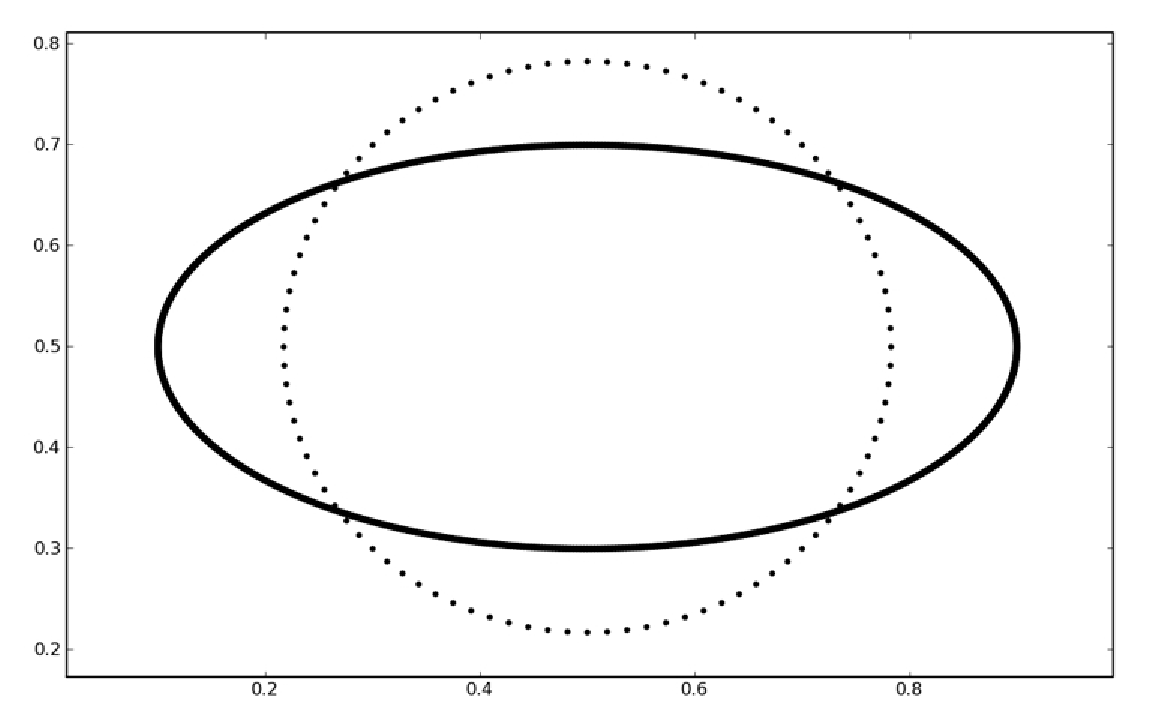
\includegraphics[bb=0in 0in 7.7in 4.8in,width=4.8in,clip]{Ellipse.pdf}
  \end{center}
  \caption{\small Initial configuration of fiber in bold and final rest configuration in dotted line.}
  \label{fig:Ellipse}
\end{figure}
Thus, the semi-implicit discretization produces the linear system
\begin{equation}
\mathbf{X}^{n+1} = \mathcal{M}_n\mathcal{A}_{h_B} \mathbf{X}^{n+1} + \mathbf{b}^n
\end{equation}
 to be solved at each time step. Equivalently, we have
\begin{equation}
(\mathit{I}- \mathcal{M}_n\mathcal{A}_{h_B}) \mathbf{X}^{n+1} = \mathbf{b}^n,
\label{eq:LinearSystem}
\end{equation}
where $\mathit{I}$ is the $2N_B\times 2N_B$ identity matrix.
The matrix $\mathit{I}- \mathcal{M}_n\mathcal{A}_{h_B}$ is symmetric and non-singular. Indeed, the argument in~\cite{TP92} for $\mathit{I}- S^*_n P_h S_n \mathcal{A}_{h_B}$ can be applied to this case as well, for suppose
\begin{align}
(\mathit{I}- \mathcal{M}_n\mathcal{A}_{h_B}) \mathbf{X} =0, \label{eq:homo}
\end{align}
then multiplying both sides of (\ref{eq:homo}) by $\mathcal{A}_{h_B}$ and taking the inner product
with $\mathbf{X}$ we get
\begin{align}
\begin{split}
0=-(\mathbf{X}, \mathcal{A}_{h_B}\mathbf{X})_{I_B} + (\mathbf{X},\mathcal{A}_{h_B}\mathcal{M}_ n\mathcal{A}_{h_B} \mathbf{X})_{I_B} &= \\
-(\mathbf{X}, \mathcal{A}_{h_B}\mathbf{X})_{I_B} + (\mathcal{A}_{h_B}\mathbf{X},\mathcal{M}_n \mathcal{A}_{h_B} \mathbf{X})_{I_B} .
\end{split}
  \label{eq:nonnegative}
\end{align}
 Both terms in the left hand side of (\ref{eq:nonnegative}) are non-negative. Therefore, it follows that each has to be equal to zero and consequently
\begin{align}
(\mathbf{X},\mathcal{A}_{h_B}\mathbf{X})_{I_B} =0. 
\end{align}
This implies that $\mathcal{A}_{h_B}\mathbf{X}=0$~\cite{TP92} and hence from (\ref{eq:homo}) we obtain that 
$\mathbf{X}=0$. Thus (\ref{eq:LinearSystem}) has a unique solution.

If the full matrix  $\mathit{M}_n$ is available (see the previous section for how to expedite its construction) it is easy to construct
simple iterative schemes to solve (\ref{eq:LinearSystem}). For example, denoting the diagonal component of $\mathit{M}_n$ by $\mathit{M}_n'$   and letting $\mathit{M}_n'' = \mathit{M}_n - \mathit{M}_n'$ we can write an iteration of weighted Jacobi type:
\begin{equation}
\mathbf{X}^{n+1,k+1} = (1-a)\mathbf{X}^{n+1,k} 
+ a(\mathit{I}- \mathit{M}_n'\mathit{A}_{h_B})^{-1}
(\mathbf{b}^n +\mathit{M}_n''\mathit{A}_{h_B}\mathbf{X}^{n+1,k}).
\label{eqn:ModJacobi}
\end{equation}
When underrelaxed, $0<a<1$, this iteration converges well, typically requiring on the order of 10 iterations to obtain
adequate residuals (on the order of the truncation error) and to maintain stability. Along the same lines, one can also consider a weighted Gauss-Seidel method of the form:
\begin{equation}
\begin{split}
\mathbf{X}^{n+1,k+1}_i
&=
(1-a)\mathbf{X}^{n+1,k} \\
&\mbox{ } +  a\left(
\frac{1}{B_{ii}} \left(\mathbf{b}^n_i - \sum_{j<i}B_{ij}\mathbf{X}^{n+1,k+1}_j-\sum_{j>i}B_{ij}\mathbf{X}^{n+1,k}_j\right)
\right)
\end{split}
\label{eqn:GaussSeidel}
\end{equation}
for $ i=1,2,\ldots,2N_B$, 
where $B=(\mathit{I}- \mathcal{M}_n\mathcal{A}_{h_B})$  and  $0<a<1$. 
While (\ref{eqn:GaussSeidel}) appears to converge slower than (\ref{eqn:ModJacobi}) in the numerical experiments
it does, however, perform well as a smoother.

The most efficient and robust approach we found to solve  (\ref{eq:LinearSystem}) is a simple algebraic multigrid. Suppose for simplicity that $N_B=2^m$ for some natural number $m$, we can then form a collection of Lagrangian grids of size $2^{m-1},2^m,\dots,2,1$, our original grid being the first level and coarser grids coming afterward.
For a given level $l$ of the multigrid hierarchy the prolongation operator $\mathcal{P}_l$ takes a fiber $\mathbf{X}_{l+1}$ at level $l+1$ and adds a node between each pair of consecutive nodes equidistant between each. As a matrix,  $\mathcal{P}_l$ has dimensions $2\cdot 2^{m-l+1}\times 2\cdot 2^{m-l}$ and has the form
\begin{equation}
\mathcal{P}_l = 
\left( \begin{array}{cccc}
1  & 0  & 0  &  \\
.5 & .5 & 0  & \dots \\
0  & 1  & 0  & \\
0  & .5 & .5 & \\
   &\vdots& & \ddots
\end{array} \right).
\end{equation}
Restriction operators are taken to be the transposes of prolongation operators. Calling $\mathcal{K}_1 = (\mathit{I}- \mathcal{M}_n\mathcal{A}_{h_B})$ we define recursively $\mathcal{K}_l = \mathcal{P}_{l-1}^{\mathit{T}} \mathcal{K}_{l-1} \mathcal{P}_{l-1}$. The Gauss-Seidel iteration (\ref{eqn:GaussSeidel}) provides a good smoother for the multigrid.
All together,  a single restriction, prolongation, and smoothing step looks like
\begin{itemize}
\item Given a guess $\mathbf{X}_l$ to the linear problem
\begin{equation}
\mathcal{K}_l\mathbf{X}_l = \mathbf{b}_l
\end{equation}
calculate the residual and restrict it to the next lowest level
\begin{equation}
\tilde{\mathbf{r}}_{l+1} = \mathcal{P}_l^T(\mathbf{b}_l - \mathcal{K}_l\mathbf{X}_l)
\end{equation}
\item Find the correction on the coarse grid by solving or approximating
\begin{equation}
\mathcal{K}_{l+1}\mathbf{X}_{l+1} = \tilde{\mathbf{r}}_{l+1}
\end{equation}
\item Correct our initial guess
\begin{equation}
\mathbf{X}_l \leftarrow \mathbf{X}_l + \mathcal{P}_l \mathbf{X}_{l+1}
\end{equation}
\item Smooth the high frequency errors in $\mathbf{X}_l$ via an underrelaxed Gauss-Seidel.
\end{itemize}
The number of iterations needed depends more on the desired degree of accuracy than a requirement for stability. Typically a single iteration of a Full Multigrid Step with one V-cycle per level is sufficient to maintain stability. 
Computationally, it appears to be preferable to use the approximate solution $\mathbf{X}^{n+1}$ we obtain from (\ref{eq:LinearSystem}) as the updated fiber position rather than applying (\ref{eq:Xt}) directly. This is because small errors in the solution to (\ref{eq:LinearSystem}) are amplified when $\mathcal{A}_{h_B}$ acts on it. 



\subsection{Results for the linear ellipse}
We present now the numerical results for the above model.
The method discussed has five primary costs. First, when constructing the implicit system (\ref{eq:LinearSystem}) we must calculate $\mathbf{b}^n$ via a fluid solve, with a cost of roughly one FE/BE. Second the cost of computing $\mathcal{M}_n$ is roughly one half FE/BE. Third is the cost of initializing the multigrid solver, calculating the coarse representations of $\mathcal{M}_n$ on the various levels of our grid. Use of sparse data structures is critical here to maintain $\mathcal{O}(N_B^2)$ cost. Fourth is the cost of our iterations to solve the linear system. Because matrix-vector multiplication is significantly cheaper than FE/BE (see table \ref{Table:MV}) a full multigrid step can be much cheaper than one FE/BE, the comparison improving as $N$ increases.
The final cost is in computing $\mathbf{u}^{n+1}$ once $\mathbf{X}^{n+1}$ is known, involving another fluid solve with cost again roughly one FE/BE. We will see that the sum of these costs results in a single timestep costing roughly 4 FE/BE; however, the stability restraint on $\Delta t$ for FE/BE will be orders of magnitude smaller than for our implicit methods, ultimately leaving us with methods substantially cheaper.

We set the elasticity constant $\sigma=10^5$ and take $N_B = 2N$. The initial configuration of the fiber is an ellipse given by
\begin{equation}
\mathbf{X}(s) = (.5 + .3\cos(2\pi sh_B), .5 + .2\sin(2\pi sh_B)).
\end{equation}
%centered at (.5,.5) with semi-major axis length $.3$ and semi-minor axis length $.2$, as in figure \ref{fig:Ellipse}.
As the simulation is run the ellipse attempts to stabilize to a circular configuration. The velocity of the fiber can reach roughly $500$ units before slowing. Taking a standard length to be the geometric mean of our radii, $.245$, we calculate the Reynolds number of our fluid to be approximately $100$.

For explicit simulations we will use an FE/BE scheme with $\Delta t$ as large as allowable while maintaining stability, which we take to be approximately $\Delta t = .00025h$. For our implicit scheme we make use of a linear multigrid with stopping criteria of $\norm{\mathbf{r}^k}_{\infty}<30\Delta t$, where $\mathbf{r}^k$ is the residual $\mathbf{b}^n-(I-\mathcal{M}_n\mathcal{A}_{h_B})\mathbf{X}^{n+1,k}$ at the $k$th iterate and $\norm{\cdot}_{\infty}$ is the sup norm. Here $\Delta t$ is taken to be close to the CFL condition, which is given approximately by $\Delta t = .02h$. The CFL restraint actually depends on $\norm{\mathbf{u}^n}_{\infty}$ as well, but we approximate $\norm{\mathbf{u}^n}_{\infty}$ at a conservative value when arriving at a formula for $\Delta t$.

The results of multiple simulations with varying $N$ for the explicit and implicit methods are given in table \ref{table:EllipseConvectiveSims}. The rows in the table correspond to identical simulation runs with different $N$. The columns under the title Explicit relate data from the FE/BE simulations, whereas the Implicit columns relate data from the implicit simulations. The two columns marked Average give the average CPU time of a single timestep. The columns marked Total give total CPU time for the entire simulation, up to a simulation time of $T=.05$.

We see that the implicit scheme costs roughly $4$ times as much per timestep, however, because $\Delta t$ can be taken up to the CFL restraint the scheme is roughly $20$ times faster than the explicit scheme in terms of total CPU time. This is a fairly modest gain. Increasing $\sigma$ does not give our implicit scheme an edge because larger $\sigma$ produces larger $\norm{\mathbf{u}^n}_{\infty}$ and hence a more restrictive CFL restraint.

Methods have been proposed to remove the CFL restraint. Alternatively if our simulations use Stokes flow then we can take arbitrarily sized timesteps with our implicit scheme while maintaining stability whereas the FE/BE method would remain mired in the same restrictive timesteps. We compare the two methods with Stokes flow in tables \ref{table:EllipseStokesSims}.

We note that caution must be used when taking large timesteps with the implicit discretizations used here. Larger timesteps lead to greater spurious currents.


\begin{table}
\caption{Ellipse relaxation for convective flows. The average CPU time per timestep and the total CPU time up to a simulation time of $T=.05$ is given. $\Delta t$ is the timestep taken and is the maximum allowed while maintaining stability.}
\label{table:EllipseConvectiveSims}
\begin{center}
\begin{tabular}{|c |c c c| c c c|}
\hline
& \multicolumn{3}{c|}{Explicit} & \multicolumn{3}{c|}{Implicit}\\
$N$ & $\Delta t$ & Average & Total & $\Delta t$ & Average & Total\\
\hline
128 & $1.95\cdot 10^{-6}$ & 0.03 & 73.35 & $1.17\cdot 10^{-4}$ & 0.10 & 4.34 \\
256 & $9.76\cdot 10^{-7}$ & 0.14 & 730.21 & $7.81\cdot 10^{-5}$ & 0.55 & 35.06\\
384 & $6.51\cdot 10^{-7}$ & 0.34 & 2613.19 & $5.21\cdot 10^{-5}$ & 1.24 & 118.98\\
512 & $4.87\cdot 10^{-7}$ & 0.63 & 6491.95 & $3.91\cdot 10^{-5}$ & 2.34 & 299.10\\
\hline
\end{tabular}
\end{center}

\caption{Ellipse relaxation for Stokes flows. The average CPU time per timestep and the total CPU time up to a simulation time of $T=.05$ is given. $\Delta t$ is the timestep taken. For the explicit scheme this is the maximum allowed while maintaining stability. The implicit scheme is unconditionally stable; the timestep taken is held constant as $N$ varies.  $^*$ denotes an extrapolated value.}
\label{table:EllipseStokesSims}
\begin{center}
\begin{tabular}{|c |c c c| c c c|}
\hline
& \multicolumn{3}{|c|}{Explicit} & \multicolumn{3}{|c|}{Implicit}\\
$N$ & $\Delta t$ & Average & Total & $\Delta t$ & Average & Total\\
\hline
128 & $1.95\cdot 10^{-6}$ & 0.03 & 683.96 & $.001$ & 0.09 & 9.34\\
256 & $9.76\cdot 10^{-7}$ & 0.15 & 7410.50 & $.001$ & 0.53 &  53.08\\
384 & $6.51\cdot 10^{-7}$ & 0.35 & $26555.30^*$ & $.001$ & 1.24 & 123.86\\
512 & $4.87\cdot 10^{-7}$ & 0.71 & $72669.41^*$ & $.001$ & 2.32 & 232.05\\
\hline
\end{tabular}
\end{center}
\end{table}



\subsection{An example of an ellipse with nonlinear $\mathcal{A}_{h_B}$}
The method used for the ellipse detailed above takes advantage of the linearity of the system (\ref{eq:LinearSystem}). This is the simplest possible test problem to consider. We consider now an example of a model ellipse with a nonlinear force and detail how to adapt the method from the above linear case.

We follow Mori and Peskin in \cite{MP2008} for the setup of our nonlinear ellipse example. In the continuous case the fiber force distribution is given by
\begin{equation}
\mathbf{F} = \frac{\partial}{\partial s} (T\mathbf{t})
\end{equation}
where $\mathbf{t}(s)$ is the tangential unit vector to $\mathbf{X}$ at $s$ and $T(s)$ is the tension at $s$ given by
\begin{equation}
T(s) = \left| \frac{\partial\mathbf{X}}{\partial s}(s) \right|
 +     \left| \frac{\partial\mathbf{X}}{\partial s}(s) \right|^2.
\end{equation}
To discretize the above we introduce difference operators. For a function $f$ defined over $\mathcal{G}_B$ we define
\begin{eqnarray}
D_s^+f(s) = \frac{f(s+1)-f(s)}{h_B},\\
D_s^-f(s) = \frac{f(s)-f(s-1)}{h_B}.
\end{eqnarray}
We then define the discrete force distribution as
\begin{equation}
\mathbf{F} = D_s^+ \left(\left(
\left| D_s^-\mathbf{X} \right| +
\left| D_s^-\mathbf{X} \right|^2 \right)
\frac{ D_s^-\mathbf{X} }{ \left| D_s^-\mathbf{X} \right| } \right).
\end{equation}
Note that there is no scalar constant $\sigma$. The stiffness in this model won't come from high fiber forces but rather small viscosity. We set $\rho = 1$ and either $\mu = .05$ or $\mu = .005$. As before the domain is $\Omega = [0,1]\times[0,1]$ which we discretize as $\Omega_h$, an $N\times N$ uniform Eulerian grid. The initial velocity of the fluid is $0$ everywhere. The fiber's initial configuration is given by
\begin{equation}
\mathbf{X}(s) = (.5 + \cos(2\pi sh_B), .5 + \sin(2\pi sh_B)).
\end{equation}
The implicit simulation attempts to solve at each time step the nonlinear system
\begin{equation}
(I - \mathcal{M}_n\mathcal{A}_{h_B})\mathbf{X}^{n+1} = \mathbf{b}^n,
\label{eqn:NonlinearSystem}
\end{equation}
where $\mathcal{M}_n$ and $\mathbf{b}^n$ are as in the linear case. The only difference here is the nonlinearity of $\mathcal{A}_{h_B}$. We could simply approximate $\mathcal{A}_{h_B}$ linearly and solve the resulting linear system. This is easily accomplished because the Jacobian $J$ of $\mathcal{A}_{h_B}$ is negative semidefinite, hence the matrix $I-\mathcal{M}_nJ$ is positive definite. Such linear approximation is simple and reasonably robust (though not unconditionally stable) and is the method employed by Mori and Peskin in their first order method. However because our methods are relatively cheap we can afford the extra stability and accuracy we obtain by solving (\ref{eqn:NonlinearSystem}) via multiple Newton iterations. At each timestep we perform Newton iterations until the sup norm of the residual is less than $10^{-4}$, typically $2$ or $3$ iterations (note that a single iteration per timestep would be identical to the linear approximation used by Mori and Peskin). The solution to the linear system obtained at each iteration of Newton's method is approximated via $3$ multigrid passes.

Although we chose this nonlinear model to allow comparison between the recent work of Mori and Peskin ~\cite{MP2008} and our own there are a few noteworthy differences between model and implementation. First, Mori and Peskin use an immersed fiber with mass while our own fiber is neutrally buoyant. And second, there are minor differences in the discretizations of the Navier-Stokes equations. Nonetheless we present the results from our numerical experiments in a format similar to that presented in ~\cite{MP2008} to facilitate comparisons.

Let $N_T$ be the number of timesteps taken, with total simulation time fixed at $1$. We fix $N_B=2N$ as before. 
In tables ~\ref{table:NonlinearEllipseSims_05CPU} and ~\ref{table:NonlinearEllipseSims_005CPU} the total CPU time is given for simulations with $\mu=.05$ and $\mu=.005$ respectively. In tables ~\ref{table:NonlinearEllipseSims_05Fluids} and ~\ref{table:NonlinearEllipseSims_005Fluids} the same times are given in terms of the cost of a FE/BE. In all four tables the columns under FE/BE hold the explicit result while the columns under $N_T=8$ and $N_T=16$ hold the implicit results, with $N_T$ as specified.




\begin{table}
\caption{Total CPU cost for the nonlinear ellipse model with $\mu=.05$. Values given are total CPU time divided by average CPU time of a single FE/BE timestep for the given $N$.}
\label{table:NonlinearEllipseSims_05Fluids}
\begin{center}
\begin{tabular}{|c|c| c c|}
\hline
$N$ & FE/BE & $N_T = 8$ & $N_T = 16$\\
\hline
$64$ & $166$ & $38.2$ & $75.5$ \\
$128$ & $500$ & $49.7$ & $89.7$ \\
$256$ & $1333$ & $53.0$ & $97.2$ \\
$512$ & $2666$ & $59.3$ & $92.6$ \\
\hline
\end{tabular}
\end{center}

\caption{Total CPU cost for the nonlinear ellipse model with $\mu=.005$. Values given are total CPU time divided by average CPU time of a single FE/BE timestep for the given $N$.}
\label{table:NonlinearEllipseSims_005Fluids}
\begin{center}
\begin{tabular}{|c|c| c c|}
\hline
$N$ & FE/BE & $N_T = 8$ & $N_T = 16$\\
\hline
$64$ & $333$ & $83.5$ & $112.4$ \\
$128$ & $1000$ & $74.8$ & $113.1$ \\
$256$ & $2666$ & $71.7$ & $112.6$ \\
$512$ & $5333$ & $59.2$ & $101.9$ \\
\hline
\end{tabular}
\end{center}

\caption{Total CPU time for the nonlinear ellipse model with $\mu=.05$.}
\label{table:NonlinearEllipseSims_05CPU}
\begin{center}
\begin{tabular}{|c|c| c c|}
\hline
$N$ & FE/BE & $N_T = 8$ & $N_T = 16$\\
\hline
$64$ & $2.94$ & $0.67$ & $1.33$ \\
$128$ & $20.89$ & $2.08$ & $3.75$ \\
$256$ & $227.85$ & $9.05$ & $16.59$ \\
$512$ & $1930.62$ & $42.94$ & $67.02$ \\
\hline
\end{tabular}
\end{center}

\caption{Total CPU time for the nonlinear ellipse model with $\mu=.005$.}
\label{table:NonlinearEllipseSims_005CPU}
\begin{center}
\begin{tabular}{|c|c| c c|}
\hline
$N$ & FE/BE & $N_T = 8$ & $N_T = 16$\\
\hline
$64$ & $5.31$ & $1.33$ & $1.79$ \\
$128$ & $42.06$ & $3.14$ & $4.75$ \\
$256$ & $455.11$ & $12.24$ & $19.22$ \\
$512$ & $3823.40$ & $42.45$ & $73.10$ \\
\hline
\end{tabular}
\end{center}
\end{table}





\section{Application; Heart Valve}
\label{Sec:valve}
We turn now to a more challenging application of the IB method. We consider a rigid valve immersed in blood flowing through an artery. The valve is indirectly restricted in motion by two hinges but is allowed to rotate. The valve, artery walls and hinges will all be modeled as immersed springs; all dynamics will be given gratis by the IB method once we provide the initial setup.

We take $\Omega=[0,2]\times[0,1]$ as our domain, again with periodic boundary conditions, which we discretize as a $2N\times N$ uniform gird. For a detail of the geometry of the problem see figure \ref{fig:ValveGeometry}. Note that the top and bottom of the artery walls include cushions in the shape of two hills. We simulate a horizontal flow through the artery by adding a forcing vector $\mathbf{f}_{j,k}=(v_{flow},0)$ to the right hand side of (\ref{eq:dmoment}), where in general $v_{flow}$ may be time dependent. This changes our explicit term $\mathbf{b}^n$ in our implicit system to
\begin{equation}
\mathbf{b}^n=\mathbf{X}^n + \Delta t\mathcal{S}^*_n\mathcal{L}_h
\left[ \mathbf{u}^n - \Delta t\mathbf{u}^n \cdot \nabla_h \mathbf{u}^n + \frac{\Delta t}{\rho} \mathbf{f} \right].
\end{equation}
\begin{figure}[!b]
  \begin{center}
    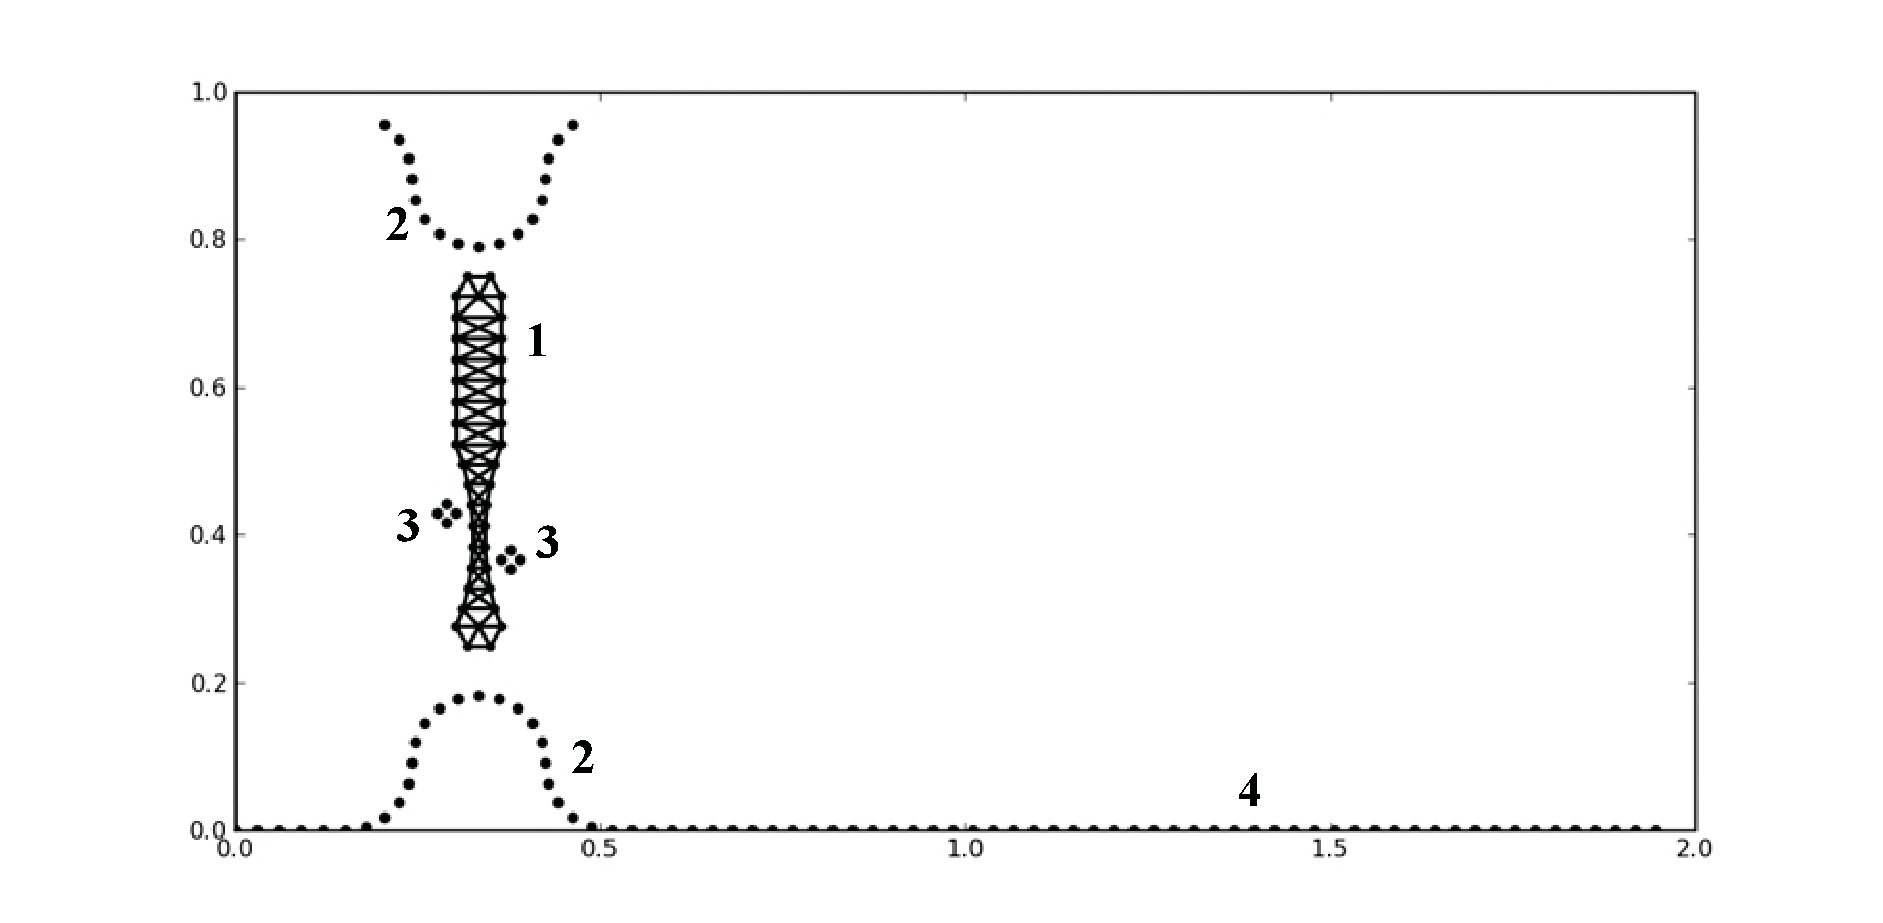
\includegraphics[bb=1in .3in 11.5in 5.85in,width=5.25in,clip]{ValveGeometry.pdf}
  \end{center}
  \caption{\small Configuration of our valve simulation. Larger nodes represent tether points. 1: Valve; 2: Cushions; 3: Hinges; 4: Artery wall}
  \label{fig:ValveGeometry}
\end{figure}
\begin{figure}[!b]
  \begin{center}
    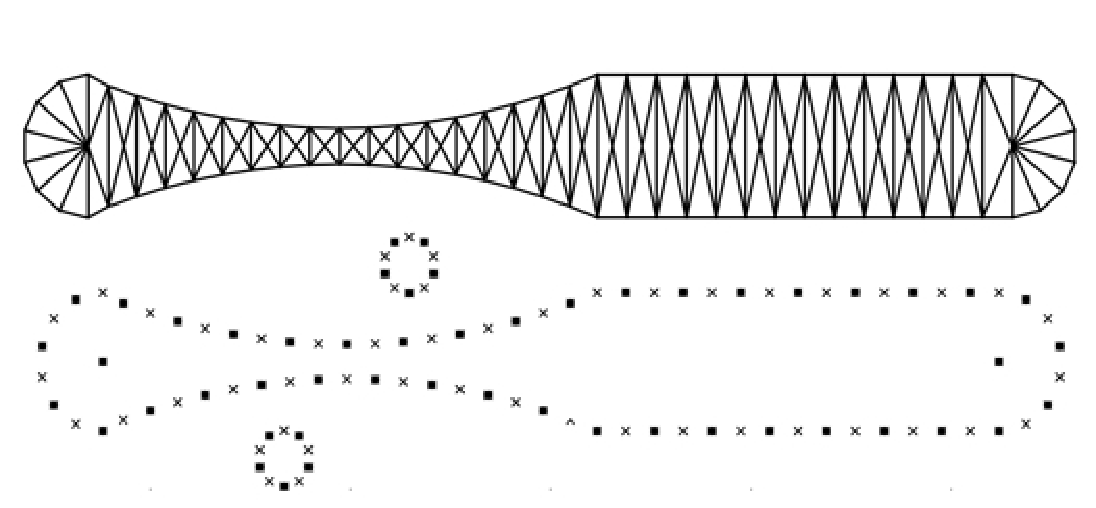
\includegraphics[bb=0in 0in 7.25in 3.3in,width=5.25in,clip]{Valve1.pdf}
  \end{center}
  \caption{\small Top: A fine grid approximation to the valve, showing only linkage. Bottom: 'x's mark the prolongation of a coarse valve marked in 'o'.}
  \label{fig:Valve1}
\end{figure}

All nodes in the wall and the two hinges are modeled as tethers, with one end of the tether fixed for all time. If $\mathbf{X}_i$ is a tethered point with base given by $\bar{\mathbf{X}}_i$ then the force generated by the tether is given by 
\begin{equation}
\mathbf{f}_i = -k_i (\mathbf{X}_i-\bar{\mathbf{X}}_i)
\label{eqn:TetherForce}
\end{equation}
where $k_i$ is the spring constant. For the body of the heart valve we will use springs between nodes. Suppose $\mathbf{X}_i$ is connected to multiple other nodes. If $\mathbf{X}_i$ is connected to $\mathbf{X}_j$ then let $k_{i,j}$ and $L_{i,j}$ be respectively the spring constant and resting length of the spring connecting them. If no connection exists between $\mathbf{X}_i$ and $\mathbf{X}_j$ then take $k_{i,j}$ to be zero. The force at $\mathbf{X}_i$ then is given by
\begin{equation}
\mathbf{f}_i = \sum_{j=1}^{N_B} -k_{i,j} \frac{\mathbf{X}_i-\mathbf{X}_j}{|\mathbf{X}_i-\mathbf{X}_j|}
(|\mathbf{X}_i-\mathbf{X}_j| - L_{i,j}).
\label{eqn:LinkForce}
\end{equation}
Note that the force operator for our ellipse given by (\ref{eqn:LinearForce}) is exactly the force given by (\ref{eqn:LinkForce}) for a loop of fiber points connected by springs with suitable spring constants and zero resting length.
For our valve though we require non-zero resting lengths in order to preserve the structure. Additionally, in order to maintain the rigidity of a solid body the spring constants must be taken very large, roughly $\mathcal{O}(10^9h^{-2})$. Similarly for the tether points representing the artery walls the spring constants must be very large to portray the tautness of the biological fibers. Because the current acts to bend the valve as it is penned between its hinges larger values of $v_{flow}$ require larger spring constants to maintain the structure. In Roma's original investigation of the problem the spring constants required to maintain rigidity forced the timesteps to be $\mathcal{O(10^{-7})}$ seconds to insure stability, with the time scales of interest roughly on the order of $1$ second. Removing this stiffness here however is not so direct as with the simpler ellipse relaxation problem. The implicit system we want to solve is still given by
\begin{equation}
\mathbf{X}^{n+1} = \mathit{M}_n\mathcal{A}_{h_B} \mathbf{X}^{n+1} + \mathbf{b}^n.
\label{eqn:Sys2again}
\end{equation}
Due to the nonzero resting lengths of the springs comprising the valve 
$\mathcal{A}_{h_B}$ isn't linear.
Unlike with the nonlinear ellipse problem however, the Jacobian $J$ of $\mathcal{A}_{h_B}$ is not semidefinite. The resulting matrix $I - \mathcal{M}_nJ$ can be shown to lack definiteness as well.

The breakdown of the definiteness of $J$ can be seen in a very simple case. Consider four immersed boundary points at $(1,0),(0,1),(-1,0),(0,-1)$, forming a square with side lengths $\sqrt{2}$ and with links connecting the perimeter of the square. We vary the resting length $l$ of the connecting springs and compute the eigenvalues of the resulting forcing function's Jacobian. The resulting eigenvalues can be seen in figure \ref{fig:BoxEigenvalues}. We see that as the resting length approaches and surpasses the side length of the square the Jacobian loses its negative semi-definiteness. This is the basic observation for most arbitrary structures. For our valve we take the resting length to be the starting length of the links comprising the valve, we thus immediately lose negative semi-definiteness once we perturb the valve structure.

Because of this the conjugate gradient method no longer converges. Biconjugate gradient method converges but may take upwards of $100$ iterations to attain a satisfactory residual. A major obstacle in accelerating convergence is that the natural preconditioner $I-\mathcal{M}_n'J$ does not capture the dynamics of our system well. Indeed a Jacobi iteration analogous to (\ref{eqn:ModJacobi}) has very poor convergence, requiring strong underrelaxation and thousands of iterations. Without adequate smoothers we can't hope for an efficient linear multigrid to solve our Newton iteration. Smoothers for the nonlinear system (\ref{eqn:Sys2again}) were likewise difficult to uncover, seemingly ruling out a nonlinear multigrid.

\begin{figure}[!b]
  \begin{center}
    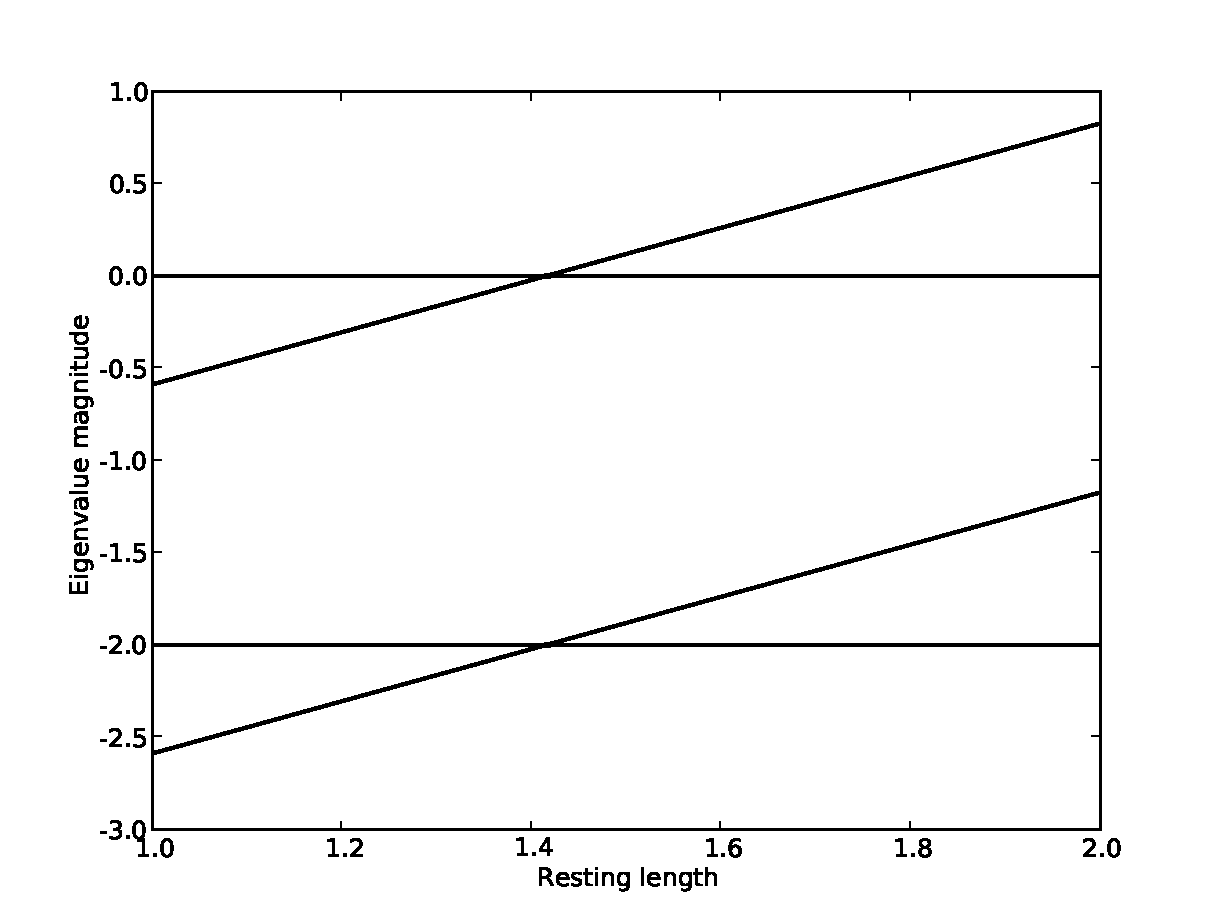
\includegraphics[bb=.15in .15in 8in 6in,width=5.25in,clip]{BoxEigenvalues.pdf}
  \end{center}

  \caption{\small Eigenvalues for the Jacobian of a fiber forcing function for four points linked as a square with varying resting length.}
  \label{fig:BoxEigenvalues}
\end{figure}

\subsection{Solving the implicit system}
Consider instead the simplest possible iterator for (\ref{eqn:Sys2again}), the fixed point iteration given by
\begin{equation}
\mathbf{X}^{n+1,k+1} = \mathit{M}_n\mathcal{A}_{h_B} \mathbf{X}^{n+1,k} + \mathbf{b}^n.
\label{eqn:fixedpoint}
\end{equation}
The first thing we observe about this iteration is that it fails spectacularly. If our initial guess is $\mathbf{X}^{n+1,0}=\mathbf{X}^n$ then $\mathbf{X}^{n+1,1}$ is the explicit update provided by a FE/BE scheme which we know to be unstable for reasonable $\Delta t$. Additional iterations of (\ref{eqn:fixedpoint}) exacerbate the instability: small errors in $\mathbf{X}^{n+1,k}$ are amplified enormously by $\mathcal{A}_{h_B}$ resulting in large errors in $\mathbf{X}^{n+1,k+1}$. In the ellipse example, this is precisely why it is preferable to use the approximate solution to (\ref{eq:LinearSystem}) as our updated configuration $\mathbf{X}^{n+1}$ rather than using (\ref{eq:uL}). Doing so provides more stability, as using (\ref{eq:uL}) is equivalent to pushing $\mathbf{X}^{n+1}$ through the fixed point iteration (\ref{eqn:fixedpoint}). Any errors present would be amplified.

The eigenvalues of $J$ are at least on the order of the spring constants comprising our valve. It should seem natural to take advantage of this by reversing the fixed point iteration (\ref{eqn:fixedpoint}). Consider the alternative fixed point iteration
\begin{equation}
\left\{
\begin{gathered}
\mathit{M}_n\mathbf{F}^{k+1} = \mathbf{X}^{n+1,k} - \mathbf{b}^n,\\
\mathcal{A}_{h_B}\mathbf{X}^{n+1,k+1} = \mathbf{F}^{k+1}.
\end{gathered}
\right.
\label{eqn:fixedpoint2}
\end{equation}
First we solve for $\mathbf{F}^{k+1}$. This is the force distribution that would move the fiber from $\mathbf{X}^n$ to $\mathbf{X}^{n+1,k}$ after a single timestep. The linear system we must solve only involves the linear positive definite operator $\mathcal{M}_n$, thus we can efficiently solve it using a multigrid. Second we determine what configuration $\mathbf{X}^{n+1,k+1}$ gives rise to this force through $\mathcal{A}_{h_B}$.
In many applications there is a unique $\mathbf{X}^{n+1,k+1}$ such that
$\mathcal{A}_{h_B}\mathbf{X}^{n+1,k+1} = \mathbf{F}^{k+1}$. For our current problem this is not the case.

To see this note that our valve is a neutrally buoyant object, detached from any fixed points, and the internal forces generated by perturbations in the valve's structure are unaffected by translation. More precisely consider two translation vectors $\mathbf{V}^1$ and $\mathbf{V}^2$ given by
\begin{gather}
\mathbf{V}^1_k = (1,0),\\
\mathbf{V}^2_k = (0,1),
\end{gather}
for any $1\leq k\leq N_B$. $\mathbf{V}^1$ and $\mathbf{V}^2$ are horizontal and vertical translation vectors, $\mathbf{X}+\mathbf{V}^1$ representing the same configuration as $\mathbf{X}$ with the valve shifted right by one unit. Shifting has no influence on the force density,
\begin{equation}
\mathcal{A}_{h_B}(\mathbf{X}+\mathbf{V}^1) = \mathcal{A}_{h_B}(\mathbf{X}+\mathbf{V}^2) = \mathcal{A}_{h_B}\mathbf{X},
\end{equation}
thus $\mathcal{A}_{h_B}$ is not injective and we may not have a unique solution to (\ref{eqn:fixedpoint2}). Indeed, $\mathcal{A}_{h_B}$ is not surjective either so (\ref{eqn:fixedpoint2}) may have no solution at all. This follows physically from conservation of momentum and angular momentum: $\mathcal{A}_{h_B}$ can't directly generate forces that move or rotate the valve. Translation and rotation can only be introduced via the fluid. 

To analyze rotation we introduce the operator $R_{\theta}$ which takes in a configuration $\mathbf{X}$ and returns the configuration obtained by rotating the valve by $\theta$ about some point. The point of rotation is arbitrary. We take it to be the center of the valve at the previous timestep,
\begin{equation}
\mathbf{x}_c = 
\left(\frac{( \mathbf{X}^n, \mathbf{V}^1)_B}{( \mathbf{V}^1, \mathbf{V}^1)_B}, 
\frac{( \mathbf{X}^n, \mathbf{V}^2)_B}{( \mathbf{V}^2, \mathbf{V}^2)_B}\right).
\label{eqn:Center}
\end{equation}
We define also
\begin{equation}
\mathbf{V}^3(\mathbf{X}) = \frac{\partial}{\partial \theta}R_\theta(\mathbf{X}). 
\label{eqn:e3}
\end{equation}
For any $1\leq k\leq N_B$ we may equivalently define $\mathbf{V}^3_k$ via
\begin{equation}
\mathbf{V}^3_k = (-Y_k+y_c,X_k-x_c)
\end{equation}
where $\mathbf{X}_k=(X_k,Y_k)$ and $\mathbf{x}_c = (x_c,y_c)$. $\mathbf{V}^3$ is the Jacobian of $R_\theta$. Note that $\mathbf{V}^3$ depends on a configuration $\mathbf{X}$. We will denote this at times by writing $\mathbf{V}^3(\mathbf{X})$.


$\mathbf{V}^1,\mathbf{V}^2,\mathbf{V}^3$ together represent three vectors outside the image of $\mathcal{A}_{h_B}$ associated with translation and rotation.
We have then that there exist solutions to (\ref{eqn:fixedpoint2}) only when $\mathbf{F}^{k+1}$ does not act to translate or rotate the valve. That is, a vector $\mathbf{F}$ lies in the image of $\mathcal{A}_{h_B}$ only when 
\begin{equation}
( \mathbf{F}, \mathbf{V}^j )_B = 0
\textrm{ for } j=1,2,3.
\label{eqn:FCondition}
\end{equation}
To see this mathematically consider the simplest case. Suppose we have only two immersed fiber points
\begin{equation}
\mathbf{X}=
\left( \begin{array}{c}
(x_1,y_1)\\
(x_2,y_2)
\end{array} \right)
\end{equation}
and there is a single link between them. Then the force they generate is
\begin{equation}
\mathbf{F}=T
\left( \begin{array}{c}
(x_2-x_1,y_2-y_1)\\
(x_1-x_2,y_1-y_2)
\end{array} \right)
\end{equation}
for some tension scalar $T$.
The rotation vector about the origin is simply 
\begin{equation}
\mathbf{V}^3=
\left( \begin{array}{c}
(-y_1,x_1)\\
(-y_2,x_2)
\end{array} \right).
\end{equation}
We have then that
\begin{equation}
( \mathbf{F},\mathbf{V}^3 )_B =
-y_1(x_2-x_1) + x_1(y_2-y_1) - y_2(x_2-x_1) + x_2(y_1-y_2) = 0.
\end{equation}
A similar calculation shows that $( \mathbf{V}^1,\mathbf{F} )_B = ( \mathbf{V}^2,\mathbf{F} )_B = 0.$
For our more complicated valve we simply have a summation of such forces, thus our forcing function must satisfy (\ref{eqn:FCondition}) where $\mathbf{F}=\mathcal{A}_{h_B}\mathbf{X}$ for any configuration $\mathbf{X}$. In general though most arbitrary vectors $\mathbf{F}$ won't satisfy (\ref{eqn:FCondition}) and we won't be able to find a solution to (\ref{eqn:fixedpoint2}). To remedy this we must factor out those components sitting outside the image of $\mathcal{A}_{h_B}$. This is easier to do with the linearized $\mathcal{A}_{h_B}$, where we may simply project onto the vector space free of the problematic vectors $\mathbf{V}^1,\mathbf{V}^2,\mathbf{V}^3$. This suggests the modified Newton iteration to approximately solve for $\mathbf{X}^{n+1,k+1}$ in (\ref{eqn:fixedpoint2}),
\begin{equation}
\left\{
\begin{gathered}
J(\mathbf{X}^{n+1,k+1,l})(\mathbf{X}^{n+1,k+1,l+1} - \mathbf{X}^{n+1,k+1,l}) = P(\mathbf{F}^{k+1} - \mathcal{A}_{h_B}\mathbf{X}^{n+1,k+1,l}),\\
\mathbf{X}^{n+1,k+1,0} = \mathbf{X}^{n+1,k}
\end{gathered}
\right.
\label{eqn:AnewtonProj}
\end{equation}
where
\begin{equation}
P(\mathbf{F}) = \mathbf{F} - \sum_{i=j}^3 \mathbf{V}^j(\mathbf{X}^{n+1,k})(\mathbf{F},\mathbf{V}^j(\mathbf{X}^{n+1,k}))_B
\label{eqn:project}
\end{equation}
is the projection operator onto rotation and translation free force distributions. Because each node in the valve is linked to only a few other nodes, $J$ is $\mathcal{O}(N_B)$ sparse. We can solve systems involving $J$ efficiently with various sparse solvers. Additionally the structure of $J$ never changes throughout a simulation, though its values do, so we may make additional optimizations in the sparse solver if desired.

Linear systems of the form $J\mathbf{X}=P\mathbf{F}$ are, strictly speaking, over determined by three degrees of freedom. To rectify this we simply isolate three degrees of freedom in $\mathbf{X}$ and fix them. These variables must be associated with the valve but are otherwise arbitrary. We could, for instance, fix the $x$ and $y$ component of a single node in the valve as well as the $x$ component of an additional node. Once fixed we may proceed to solve for $\mathbf{X}$ such that $J\mathbf{X}=P\mathbf{F}$ is satisfied at all other free points. What is important, however, is that iterations of (\ref{eqn:AnewtonProj}) in such a manner will converge to an $\mathbf{X}$ that satisfies $\mathcal{A}_{h_B}\mathbf{X}=P\mathbf{F}$ at all points, even those we fixed. In this sense we arrive at an updated configuration $\mathbf{X}^{n+1,k+1}$ which satisfies (\ref{eqn:fixedpoint2}) up to components outside the image of $\mathcal{A}_{h_B}$.

Iterations of (\ref{eqn:fixedpoint2}) typically provide square convergence. The limit need not be, and usually isn't, a solution to (\ref{eqn:Sys2again}). The limit is, however, a stable update for our configuration $\mathbf{X}$. As an aside, it is important to note that this iteration converges precisely because the standard fixed point iteration (\ref{eqn:fixedpoint}) diverges. As we modify the parameters of our simulation though, for instance if we were to drastically decrease the spring constants, then (\ref{eqn:fixedpoint}) may converge whereas (\ref{eqn:fixedpoint2}) would diverge. There are, moreover, instances with mixed spring constants, both large and small, where neither iteration converges. Removing the crosslinks of our valve is one such example (and is an example of a broader class of ill-posed problems).
For our case with large spring constants everywhere there is no problem, (\ref{eqn:fixedpoint}) converges rapidly. Indeed increasing the spring constants aids in the convergence.

Of course this iteration, as it is currently formulated, does not allow for translation or rotation of our valve. Thus, while it may provide stable updates it does not lead to physically acceptable simulations. We must somehow reintroduce translation and rotation in our simulation.
The simplest method to do this is to use the location and angle of the valve configuration obtained from an explicit update. To accomplish this we may simply take our initial guess $\mathbf{X}^{n+1,0}$ for iterations of (\ref{eqn:AnewtonProj}) to be
\begin{equation}
\mathbf{X}^{n+1,0} = R_{\theta}\mathbf{X}^n + \mathbf{V}^1(\tilde{\mathbf{X}}-\mathbf{X}^n,\mathbf{V}^1)_B
+ \mathbf{V}^2(\tilde{\mathbf{X}}-\mathbf{X}^n,\mathbf{V}^2)_B
\label{eqn:InitialGuess}
\end{equation}
where
\begin{equation}
\theta = (\tilde{\mathbf{X}}-\mathbf{X}^n
-\mathbf{V}^1(\tilde{\mathbf{X}}-\mathbf{X}^n,\mathbf{V}^1)_B
-\mathbf{V}^2(\tilde{\mathbf{X}}-\mathbf{X}^n,\mathbf{V}^2)_B
,\mathbf{V}^3(\mathbf{X}^n))_B
\end{equation}
and
\begin{equation}
\tilde{\mathbf{X}} = \mathbf{X}^n + \mathcal{M}_n\mathcal{A}_{h_B}\mathbf{X}^n
\end{equation}
is the FE/BE update prediction. Here we are taking the FE/BE prediction for the following timestep $\tilde{\mathbf{X}}$ and extracting its location and angle. We then take our current configuration $\mathbf{X}^n$ and modify the location and angle of the valve to match that in $\tilde{\mathbf{X}}$. Afterward we may proceed to apply iterations of (\ref{eqn:AnewtonProj}) and since this doesn't introduce translation or rotation we will maintain the location and angle we extracted from the FE/BE prediction.

Other predictors may be employed as well. 
For instance we may rediscretize our problem on a coarser grid, solve for the updated timestep, prolong the solution to our original fine grid and extract its gross properties. In fact solving (\ref{eqn:fixedpoint2}) via iterations of (\ref{eqn:AnewtonProj}) is a good nonlinear smoother, opening the possibility for a nonlinear multigrid. Other predictors may involve higher order explicit update mechanisms for computing $\tilde{\mathbf{X}}$ or treating the valve as a true rigid body and predicting its motion through rigid body dynamics.

\subsection{Reintroducing translation and rotation iteratively}
Many of these explicit predictions behave quite satisfactorily and in conjunction with (\ref{eqn:fixedpoint2}) provide accurate and stable solutions to (\ref{eqn:Sys2again}). In many applications this is sufficient. If we perform iterations of (\ref{eqn:AnewtonProj}) after using the initial guess (\ref{eqn:InitialGuess}) we can obtain an approximate solution to (\ref{eqn:Sys2again}) with error on the order of the accuracy of our discretization.

In our particular simulation, however, extra care must be taken. The close proximity of the valve to its hinges can quickly lead to unphysical collisions 
if small errors in translation propagate throughout the simulation. 
This proximity can also seriously affect the behavior of an explicit prediction, leading to wild translation and rotation. We thus seek a means to reintroduce the three degrees of freedom we have neglected in applying (\ref{eqn:fixedpoint2}).

Suppose that we have a solution $\mathbf{X}^{n+1}$ to our system (\ref{eqn:Sys2again}). We must have then
\begin{equation}
( \mathbf{F}^{n+1}, \mathbf{V}^j(\mathbf{X}^{n+1}) )_B = 0
\textrm{ for } j=1,2,3.
\label{eqn:FCondition2}
\end{equation}
where $\mathbf{F}^{n+1}$ is such that 
\begin{equation}
\mathcal{M}_n\mathbf{F}^{n+1}=\mathbf{X}^{n+1}-\mathbf{b}^n.
\end{equation}
This is because if $\mathbf{X}^{n+1}$ solves (\ref{eqn:Sys2again}) then $\mathbf{F}^{n+1} = \mathcal{A}_{h_B}\mathbf{X}^{n+1}$ and $\mathcal{A}_{h_B}$ can't generate forces with nonzero components along $\mathbf{V}_j$, $j=1,2,3$.
(\ref{eqn:FCondition2}) suggests that before every iteration of (\ref{eqn:fixedpoint2}) we simply shift and rotate $\mathbf{X}^{n+1,k}$ such that 
$( \mathbf{F}^{k+1}, \mathbf{V}_j(\mathbf{X}^{n+1,k}) )_B = 0$ for $j=1,2,3$, where $\mathcal{M}_n\mathbf{F}^{k+1}=\mathbf{X}^{n+1,k}-\mathbf{b}^n$ as before. This can be approximately accomplished by finding $(a_1,a_2)$ and $\theta$, a translation vector and an angle, such that for $j=1,2,3$
\begin{equation}
( \mathcal{M}_n^{-1}(\mathbf{X}^{n+1,k}+a_1\mathbf{V}^1+a_2\mathbf{V}^2+\theta\mathbf{V}^3(\mathbf{X}^{n+1,k})-\mathbf{b}^n),  \mathbf{V}^j(\mathbf{X}^{n+1,k}) )_B = 0.
\label{eqn:ProjFree}
\end{equation}
Or, equivalently,
\begin{equation}
\left( \begin{array}{ccc}
(\mathbf{W}^1,\mathbf{V}^1)_B &
(\mathbf{W}^2,\mathbf{V}^1)_B &
(\mathbf{W}^3,\mathbf{V}^1)_B \\
(\mathbf{W}^1,\mathbf{V}^2)_B &
(\mathbf{W}^2,\mathbf{V}^2)_B &
(\mathbf{W}^3,\mathbf{V}^2)_B \\
(\mathbf{W}^1,\mathbf{V}^3)_B &
(\mathbf{W}^2,\mathbf{V}^3)_B &
(\mathbf{W}^3,\mathbf{V}^3)_B \\
\end{array} \right)
\left( \begin{array}{c}
a_1 \\ a_2 \\ \theta
\end{array} \right)
=
-\left( \begin{array}{c}
(\mathbf{F}^{k+1},\mathbf{V}^1)_B \\
(\mathbf{F}^{k+1},\mathbf{V}^2)_B \\
(\mathbf{F}^{k+1},\mathbf{V}^3)_B \\
\end{array} \right),
\end{equation}
where $\mathcal{M}_n\mathbf{W}^j = \mathbf{V}^j$ for $j=1,2,3$.
We then construct an updated configuration 
\begin{equation}
\mathbf{X}^{n+1,k} \leftarrow R_{\theta}\mathbf{X}^{n+1,k}+a_1\mathbf{V}^1+a_2\mathbf{V}^2
\label{eqn:Rotate}
\end{equation}
after which we proceed to calculate $\mathbf{X}^{n+1,k+1}$ via (\ref{eqn:AnewtonProj}) using an unmodified $\mathbf{F}^{k+1}$.
In this manner we obtain an iteration which converges rapidly to a solution of (\ref{eqn:Sys2again}).
This iteration converges nearly as quickly as (\ref{eqn:fixedpoint2}) does for a fixed valve with no rotation or translation. There is an additional cost per iteration though. The predominant costs come from solving linear systems involving $\mathcal{M}_n$, which we must now do four times, calculating $\mathbf{F}^{k+1}$ as well as $\mathbf{W}^j$ for $j=1,2,3$.

Luckily these costs aren't great in practice. $\mathbf{W}^1$ and $\mathbf{W}^2$ only need to be calculated once per timestep. For our simulations we calculate $\mathbf{W}^3$ only once per timestep as well, even though $\mathbf{V}^3$ depends on the current guess $\mathbf{X}^{n+1,k}$. We found that this did not degrade the final residual beyond the limits of accuracy provided by our multigrid solver.
Additionally $\mathbf{W}^j$ for $j=1,2,3$ will not change greatly from timestep to timestep, precipitating their use as good initial guesses in the following timesteps. Together the actual costs of our iterators are not the predominant cost of each timestep but are rather dominated by the cost of initializing the linear system and multigrid itself.

There is an additional subtlety that we wish to point out. The prolongation and restriction operators we use in our multigrid for solving $\mathcal{M}_n^{-1}$ are geometrically inspired, relying on the underlying structure of our configuration. However this fails to give adequate weight to the fluid interactions \textit{between} surfaces, in particular the interaction between the ends of the valve and the cushions as well as the interaction between the middle of the valve and the hinges.

In our case the multigrid still converges but not sufficiently quickly at key points. In particular with only a few iterations our multigrid may fail to capture all the necessary dynamics between the valve and hinges to prevent collision and protrusion. Certainly a more robust algebraic multigrid algorithm for selecting prolongation and restriction operators may solve this. Keeping with the mentality of a geometric multigrid however we simply employ a quick yet effective alteration to our smoother.

We maintain our standard Gauss-Seidel iteration, however, in addition we also perform a direct solve via Gaussian elimination of a subset of our problem. Because we are only concerned with the high accuracy needed to prevent collision between the valve and hinge we isolate those points close to the hinge. See figure \ref{fig:Box}. Holding all other points outside this region fixed we then proceed to solve the resulting reduced system. Afterward we perform the standard Gauss-Seidel iteration to smooth the interface between the points inside and outside the solved region. Because the number of points we are solving for is relatively small this procedure is quite cheap and doesn't contribute greatly to the cost of the multigrid iteration.
 
As an aside, note that even with exact solutions to (\ref{eqn:Sys2again}) taking $\Delta t$ large may still produce collisions due to inaccuracies in the discretization itself, rather than any shortcomings in our methods to solve the implicit systems. Nonetheless in such cases the exact solution to the implicit system (\ref{eqn:Sys2again}) will still behave much more satisfactorily than with explicit updates for the valve location and angle.

\begin{figure}[!b]
  \begin{center}
    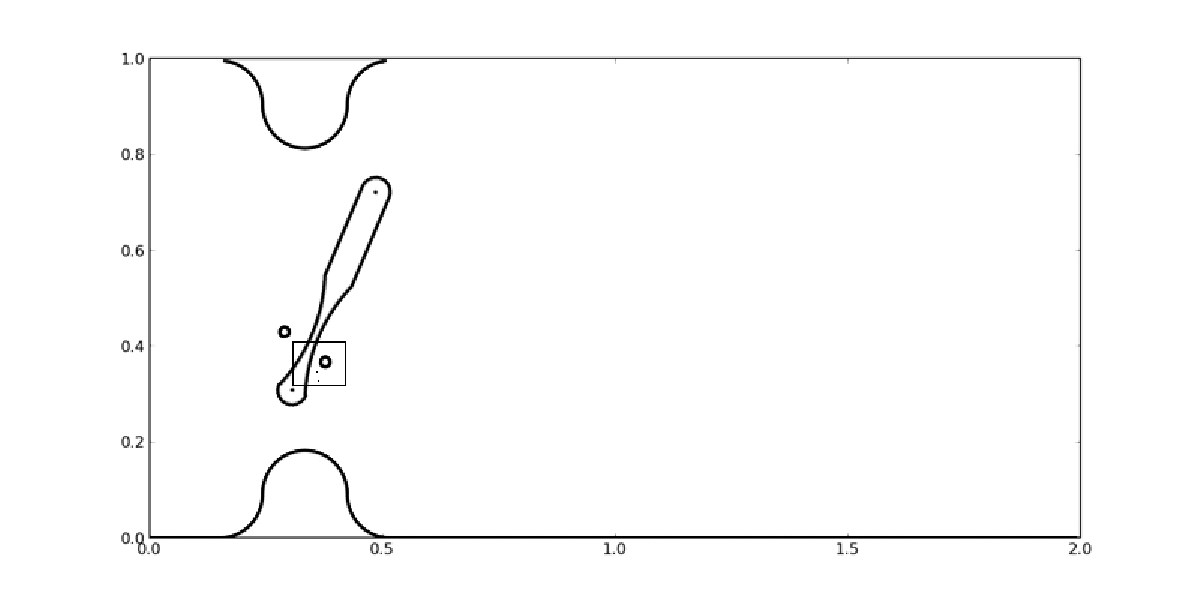
\includegraphics[bb=.5in .25in 7.35in 3.75in,width=5.25in,clip]{Box.pdf}
  \end{center}

  \caption{\small Configuration of our valve system after some period of time. The small box contains the subsystem of fiber points we solve exactly.}
  \label{fig:Box}
\end{figure}


\section{Results for the application to the heart valve}
For our heart valve simulation the initial condition is a rest configuration of all links and tethers. The valve rests between the two hinges and is parallel to the $y$-axis. The current force is $v_{flow}=100$ and all spring constants are taken to be $10^9l^{-2}$, where $l=h/2$ is the length between nodes in our valve. We have much slower velocities here than in the ellipse relaxation, with speeds reaching roughly $10$ units. Taking a characteristic length to be the length of the heart valve we obtain a Reynolds number of roughly $5$. The slower speeds lead to a CFL restraint orders of magnitude larger and this allows our implicit scheme to show its power, even though now $N_B \approx 4N$, leading to an implicit timestep costing roughly $20$ times that of an explicit one.

For the FE/BE simulation $\Delta t$ is again taken to be the maximum allowable, with $\Delta t = 30h\sigma^{-2}$. For our implicit scheme we fix $\Delta t=.0025$, well below the CFL restraint. The results for the explicit simulations are given in table \ref{table:ValveFEBESims} with the results from the implicit simulations following in table \ref{table:ValveImplicitSims}.

Here the CFL restraint is much less restrictive than in the linear ellipse relaxation problem. The implicit scheme thus fairs much better compared to FE/BE. The total CPU time is on the order of $1000$ times less, three orders of magnitude. $\Delta t$ may be taken even larger, up to the CFL restraint, leading to even greater savings in CPU time, but this will typically increase leakage through the immersed boundary and eventually allow the valve to collide and pass through the hinges.

\subsection{Time dependent $v_{flow}$}
The purpose of $v_{flow}$ is to impart a force on the fluid which leads to the valve opening and closing. If $v_{flow}$ is held constant we can only open the valve. To then close the valve we must introduce a time dependent $v_{flow}$.
We define
\begin{equation}
v_{flow}(t) =
\left\{
\begin{array}{cccc}
&60000t(.1-t)& &t<.1 \\
&-60000(t-.1)(.2-t)& &t\geq .1
\end{array}
\right. .
\label{eqn:VariableFlow}
\end{equation}
Solving the resulting numerical problem is typically more difficult with explicit methods; however, for our implicit methods no changes to the code are required except to directly account for the changing values of $v_{flow}$. We demonstrate the time evolution of the system in figure \ref{fig:TimeProgression}.

\begin{table}
\caption{The number of Lagrangian nodes $N_B$ and the maximum stable timestep $\Delta t$ for a FE/BE method are given for increasing values of $N$.}
\label{table:ValveSimData}
\begin{center}
\begin{tabular}{|c|c c|}
\hline
$N$ & $N_B$ & $\Delta t$ \\
\hline
128 & 520 & $1.15\cdot 10^{-7}$ \\
256 & 1053 & $2.89\cdot 10^{-8}$ \\
384 & 1592 & $1.29\cdot 10^{-8}$ \\
512 & 2122 & $7.24\cdot 10^{-9}$ \\
\hline
\end{tabular}
\end{center}

\caption{Heart valve simulation with Forward Euler/Backward Euler scheme. The total CPU time taken to run the simulation up to time $T$ is given, with the average CPU time per timestep given. $^*$ denotes an extrapolated value.}
\label{table:ValveFEBESims}
\begin{center}
\begin{tabular}{|c|c c c c c|}
\hline
$N$ & Average & $T=.01$ & $T=.05$ &$T=.1$ &$T=.5$\\
\hline
128 & .024 & 2110.49 & 10508.95 & $21017.90^*$ & $105089.54^*$ \\
256 & .109 & $37687.16^*$ & $188435.83^*$ & $376871.66^*$ & $1884358.32^*$ \\
384 & .249 & $193168.57^*$ & $965842.85^*$ & $1931685.70^*$ & $9658428.53^*$ \\
512 & .503 & $694291.69^*$ & $3471458.49^*$ & $6942916.98^*$ & $34714584.93^*$\\
\hline
\end{tabular}
\end{center}

\caption{Heart valve simulation with implicit scheme. The total CPU time taken to run the simulation up to time $T$ is given, with the average CPU time per timestep given. $\Delta t = .0025$.}
\label{table:ValveImplicitSims}
\begin{center}
\begin{tabular}{|c|c c c c c|}
\hline
$N$ & Average & $T=.01$ & $T=.05$ &$T=.1$ &$T=.5$\\
\hline
128 & .588 & 2.001 & 10.436 & 21.155 & 117.767\\
256 & 2.014 & 7.640  & 38.171 & 76.297 & 402.749\\
384 & 4.747 & 18.735 & 93.266 & 186.270 & 949.409\\
512 & 9.538 & 34.984 & 174.702 & 348.531 & 1907.635\\
\hline
\end{tabular}
\end{center}
\end{table}

\begin{figure}[p]
\begin{center}
%\includegraphics[bb=1.3in .5in 13.5in 6in,width=4.2in,clip]{fig_c10_n512.pdf}
%\hfill
\includegraphics[bb=1.3in .5in 13.5in 6in,width=4.2in,clip]{fig_c25_n512.pdf}
\hfill
\includegraphics[bb=1.3in .5in 13.5in 6in,width=4.2in,clip]{fig_c45_n512.pdf}
\hfill
\includegraphics[bb=1.3in .5in 13.5in 6.3in,width=4.2in,clip]{fig_c70_n512.pdf}
\hfill
\includegraphics[bb=1.3in .5in 13.5in 6.5in,width=4.2in,clip]{fig_c80_n512.pdf}
\end{center}
\caption{\small Vorticity field of our valve system through time. $N=512,N_B=2082,\Delta t=.0025,\sigma=2.62\cdot 10^{14}$. Frames shown at total simulation time $T=0.0625,0.1125,0.1750,0.2000$}
\label{fig:TimeProgression}
\end{figure}






\section{Conclusion}
Implicit methods for alleviating the stiffness of the IB method have been around for some time. Their implementation involves solving systems of equations typically thought to be prohibitively expensive. Our intent with this paper was to illuminate paths to solving the systems arising from certain semi-implicit discretizations of the IB method. We have provided avenues to this end for two particular applications of the IB method but there will likely remain challenges when applying the techniques detailed here to the incredibly varied body of applications for which the IB method is implemented.

A key benefit of our methods is that they have no dependence on the specifics of the fluid solver $\mathcal{L}_h$. If we use an adaptive mesh to achieve fluid solves in $\mathcal{O}(N_B)$ time then this will carry over to our implicit solvers, allowing us to take arbitrary time steps with the minimal order cost possible. This is a particularly exciting prospect for 3D cases and is a current aim of our own ongoing research.



\bibliographystyle{elsarticle-num}
\bibliography{interface}


%\begin{thebibliography}{00}

% \bibitem{label}
% Text of bibliographic item

%\bibitem{}

%\end{thebibliography}

\end{document}


% The Appendices part is started with the command \appendix;
% appendix sections are then done as normal sections
% \appendix

% \section{}
% \label{}
